\setcounter{chapter}{1}
\chapter{The \hisparc detection station}

% What type of detectors are used (and why), and why organised in independent stations
The \hisparc experiment utilizes independent detection stations which use multiple scintillator detectors to perform standalone triggering. A set of scintillator detectors connected to the same readout system are called a station. Since each station performs its own triggering, stations do not need to be interconnected. For stations separated by large distances this approach is more practical, since wireless and wired communication are either to unreliable or to slow. For experiments like Auger, where the space between individual surface detectors is mostly empty, wirelessly connecting them is an option. A \hisparc station consists of either 2 or 4 scintillator detectors connected to \hisparc electronics. In this chapter the specifications and performance of a station is discussed. First the scintillator detectors are described in detail, followed by the electronics which perform the readout and triggering. Finally the way it all works together is looked at.

% Mention the optional weather station.
In addition to the scintillator detectors a station may also have weather sensors. These are readout with a console which sends the data to the PC. The weather data is used to examine the environmental effects on the scintillator detectors and the air showers. The weather station is also explained.


\section{Scintillator detector}

% Using scintillators with PMTs provide good particle detection efficiency, \SI{100}{\percent} of energetic leptons are detected, also some gammas are seen.
The scintillator detector consists of two main components which perform the detection. The scintillator sheet, which emits light when charged particles pass through it, and the photomultiplier tube (\pmt) which converts the scintillation photons into an electric signal. In \cref{fig:scintillator_detector} a scintillator detector in the process of being built is shown.

\begin{figure}
    \centering
    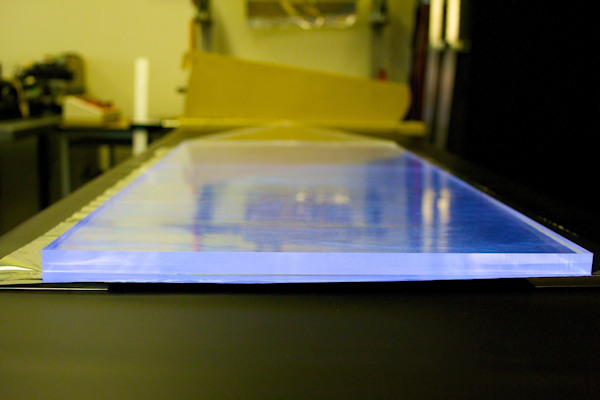
\includegraphics[width=0.6\textwidth]
                    {plots/station/ADL_115651.jpg}
    \caption{A photo of a partially finished scintillator detector. The scintillator sheet is prepared to be wrapped in aluminium foil, followed by the pond foil.}
    \label{fig:scintillator_detector}
\end{figure}


\subsection{Scintillator detector components}

% Scintillator size and material
Plastic scintillators have been selected as detection material. This is a relatively cheap material with high reliability and excellent efficiency. The scintillator is a sheet of \SI[product-units=power]{100 x 50 x 2}{\centi\meter} made from BC-408 \cite{sgc2011bc408}. The BC-408 material has good timing properties and light output for charged particles. The wavelength of maximum emission is \SI{425}{\nano\meter} (violet).

% PMT size and type
The chosen photomultiplier tube \cite{et2010pmt,hamamatsu2014pmt} is a compact \SI{29}{\milli\meter} (\SI{25}{\milli\meter} effectively) diameter and approximately \SI{11}{\centi\meter} long (the final length depends on the connected power supply) \pmt. The photocathode material is biakali, which has a quantum efficiency of \SI{25}{\percent} for the wavelength of maximum emission of the scintillator. The \pmts contain 11 high-gain caesiated antimony (SbCs) dynodes. The \pmts are very efficient at amplifying faint light pulses to measurable electric signals. Several brands and types of \pmts have been used. At first \pmts (including power supply) were sourced from Electron Tubes, ET Enterprises and \senstech. Later new \pmts were constructed using Hamamatsu tubes with a \nikhef power supply. The \nikhef \pmt power supply is also compatible with the previously used tubes and can be used to replace failed power supplies.

Besides these the scintillator detector construction consists of several other components. An isosceles triangle with a flat top made from polymethylmethacrylate (PMMA) is used as light guide. The light guide has the following measurements a base of \SI{50}{\centi\meter}, legs of \SI{71.5}{\centi\meter}, the thickness is \SI{2.2}{\centi\meter}, and the width of the top is also \SI{2.2}{\centi\meter}. The light guide is glued to the scintillator using Optical Cement \cite{sgc2014bc600}. A little adapter piece from square to round shape (same material as light guide) is attached to the square top of the triangle with Optical Cement and the round window of the \pmt with optical tape [ref type?]. This construction is wrapped in thin, \SI{30}{\micro\meter}, aluminium foil. The corners of the scintillator are covered with patches of thicker aluminium foil to prevent the sharp edges from piercing the foil. This is then wrapped in \SI{0.5}{\milli\meter} thick light-tight black pond foil to keep light out and protect the aluminium foil from outside influences.

% Material is mostly 'off the shelf'. Construction/assembly can be performed by students.
All components are readily available, off the shelf, from suppliers and not specifically designed for \hisparc.

\begin{figure}
    \centering
    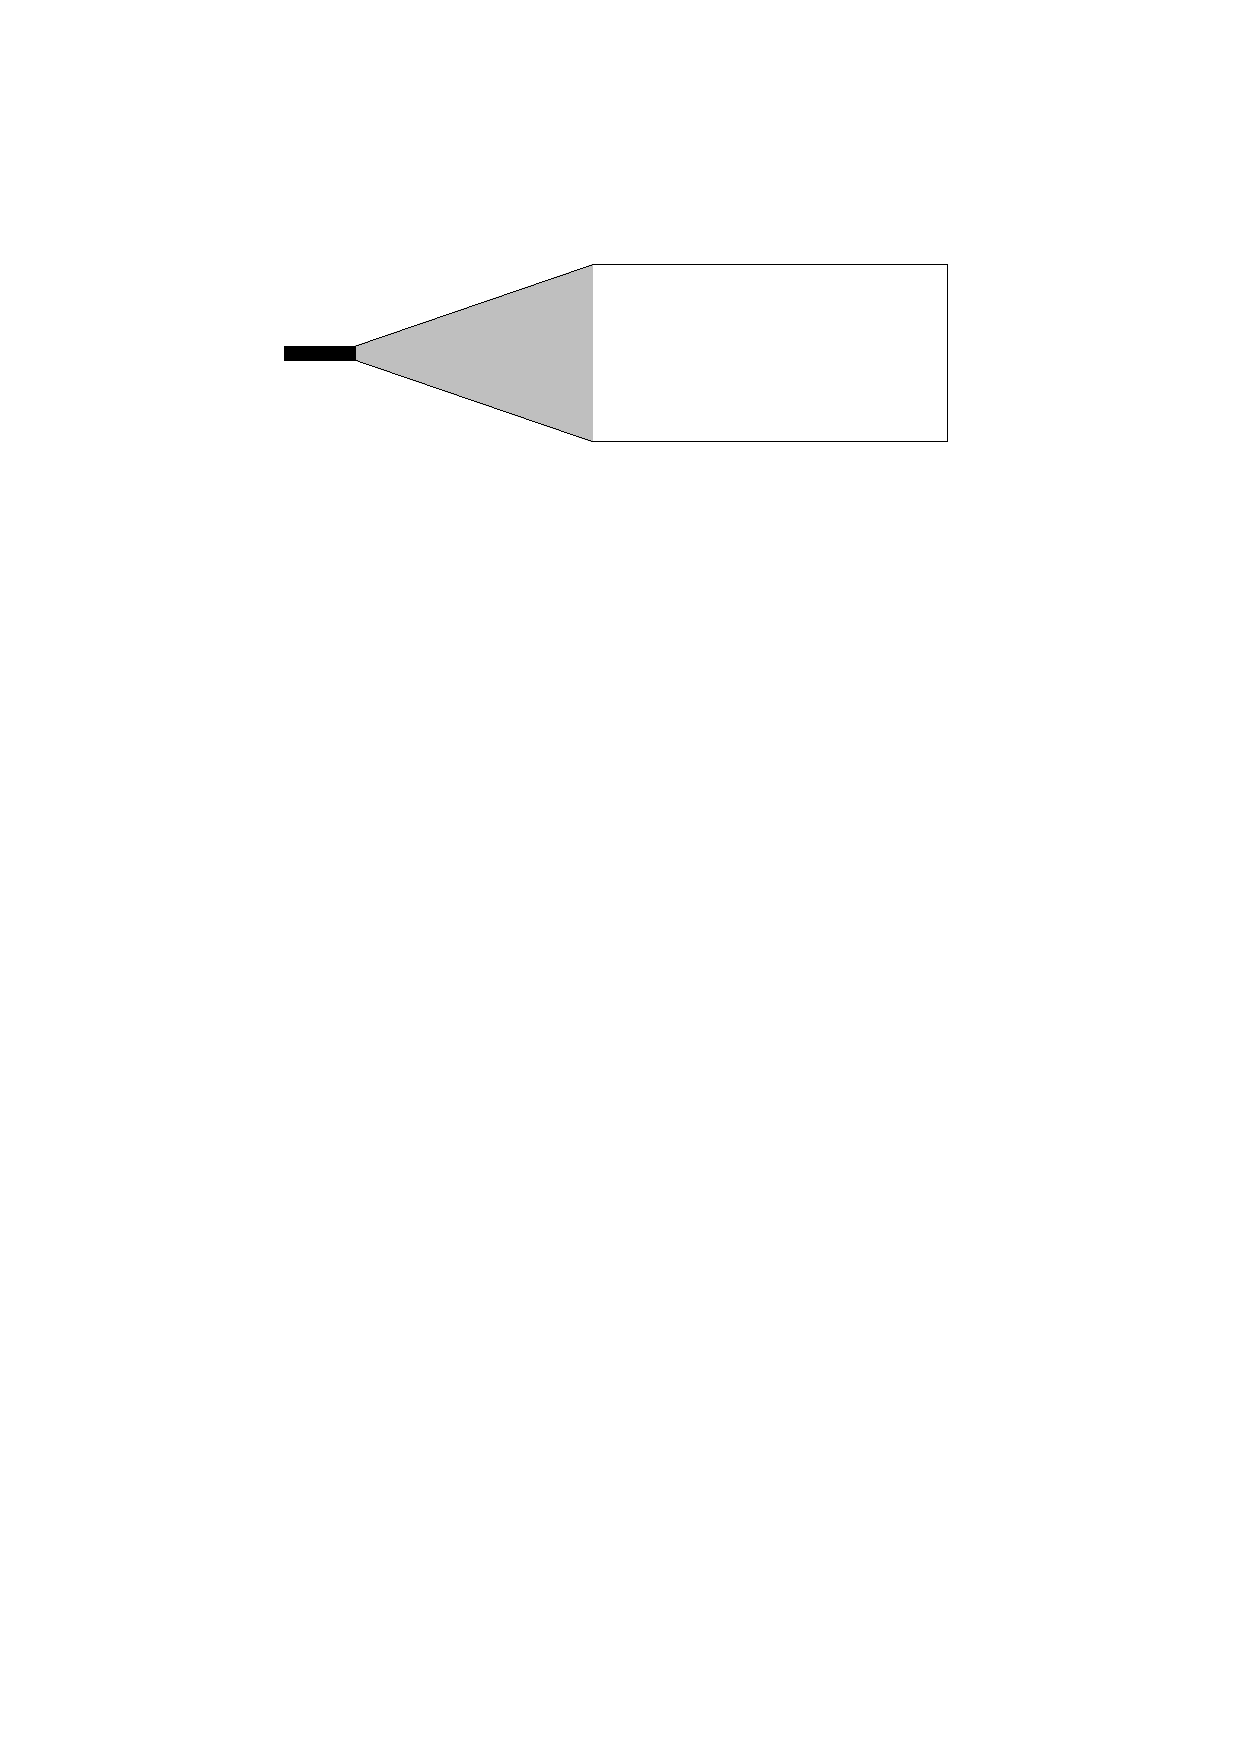
\includegraphics[width=0.6\textwidth]
                    {plots/station/schematic_detector}
    \caption{A schematic of the detector, the various components are indicated.}
    \label{fig:schematic_detector}
\end{figure}

% Detector is protected by skibox from weather and is secured in place by weights.
The complete scintillator detector dimensions are (approximately) \SI[product-units=power]{200 x 50 x 3}{\centi\meter} and fit well in the chosen detector casing, namely roof boxes (in Dutch generally referred to as `ski box'). These can be securely fastened and are designed to withstand all kinds of weather. Access to the scintillator detector for maintenance is also easy. Also with maintenance in mind, the optical tape with which the \pmt is attached allows it to be easily replaced. In \cref{fig:detector_in_skibox} a scintillator detector in a skibox is shown.

\begin{figure}
    \centering
    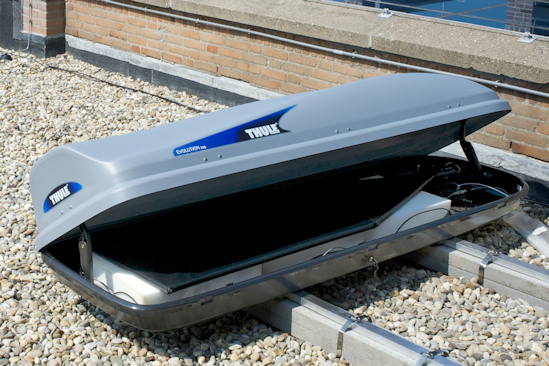
\includegraphics[width=0.6\textwidth]
                    {plots/station/ADL_105036.jpg}
    \caption{Scintillator detector in a skibox on the roof.}
    \label{fig:detector_in_skibox}
\end{figure}


\subsection{Scintillation light}

% How Scintillator works
Charged particles lose energy in the scintillator in interactions with the base of the scintillator, polyvinyltoluene. Ionisation is the main source of energy loss for energetic charged particles (electrons, muons). The base will emit photons which are rapidly absorbed by the fluor of the scintillator, anthracene. The fluor then emits light at a lower wavelength, to which the scintillator is more transparent. Some of this light will reach the \pmt.

% Most shower muons/electrons are minimum ionising particles (mips) and have similar energy loss in the detectors, given by Bethe-Bloch (spread on energy loss given by Landau).
The average energy deposited by the particle going through the scintillator is described by the Bethe-Bloch formula [ref]. This gives the amount of energy lost by the particles per \si{\gram\per\centi\meter\squared} of the material it passes through. The used scintillator has a density of \SI{1.032}{\gram\per\centi\meter\cubed} and thickness of \SI{2}{\centi\meter}. So a particle going vertically through the scintillator passes through about \SI{2}{\gram\per\centi\meter\squared}. However, the interactions in which the particles lose energy is a statistical process, the energy loss is not a fixed number but a distribution, the Landau distribution [ref]. The ionisation energy loss (predicted by Bethe-Bloch) for both electrons and muons reaches a minimum value at some point. Muons and electrons at this energy (\SI{325e6}{\eV} and \SI{e6}{\eV} respectively) are referred to as \textit{minimum ionising particles} (\mip). In \cref{fig:bethe-bloch} the energy loss for electrons and muons is shown as a function of their energy. Shown are the total losses (grey), losses due to ionisation (black), and other loss processes. The ionisation losses are the only ones of real interest, since those result in the detectable scintillation light.

% Energy loss is approximately: 2 MeV g^-1 cm^2 * 1.032 g cm^-3 * 2 cm
% Energy per scintillation photon: h*c/325 nm = 3.8149 eV
% Number of scintillation photons: ...
% Fraction that reaches \pmt (before photocathode): ...
% Where is energy 'lost'? in base -> fluor?

\begin{figure}
    \centering
    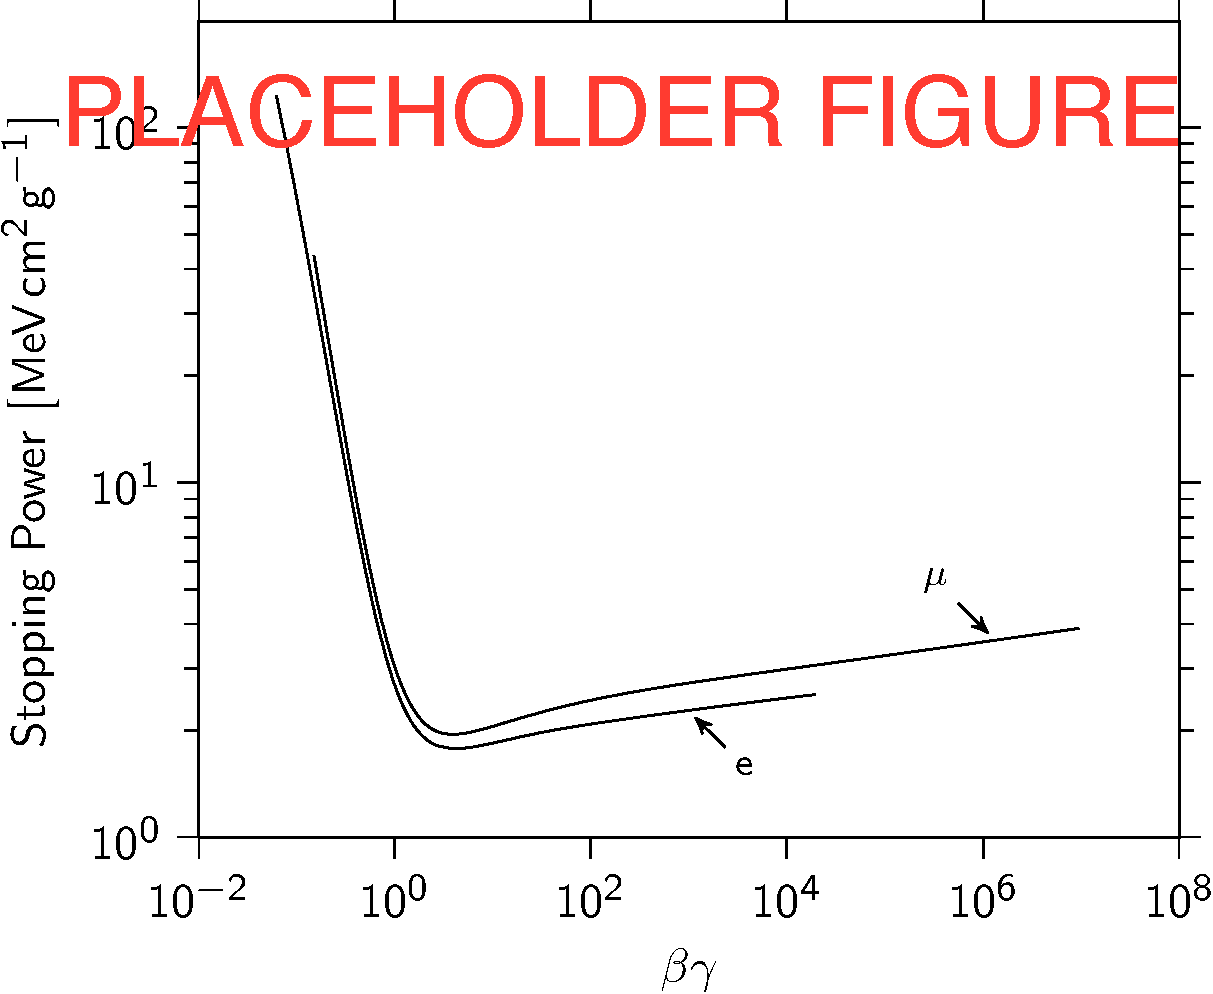
\includegraphics[width=0.6\textwidth]
                    {plots/station/bethe-bloch}
    \caption{Expected ionisation energy loss in the scintillator for electrons and muons as a function of their energy. Calculated with the Bethe-Bloch formula for the used scintillation material. [use eV[/c] horizontal scale (two scales?) or keep beta gamma. and add other losses?]}
    \label{fig:bethe-bloch}
\end{figure}

The scintillator is \SI{2}{\centi\meter} thick, however, many particles have a longer path through it because they travel at an angle. This increases the expected mean energy loss. The path could also be shorter if the particle passes through one of the sides of the scintillator, but due to the large area of the scintillator relative to its thickness the chance of that happening is low.


\subsubsection{Gammas in the scintillator}

Energetic photons (\SI{>100}{\keV}) can also deposit energy in the scintillator due to Compton scattering and pair creation \cite{lio2015}. However, the cross sections for these interactions is very low. A \SI{e6}{\eV} photon has a mean free path greater than \SI{10}{\centi\meter}, which increases further for higher energy photons. Despite the low detection chance, the large number of photons in an air shower makes them statistically relevant.

In case of Compton scattering electrons are `kicked' free by the photon, the energy transferred to the electron will cause scintillation light to be produced, as described above, the amount depends on the energy of the electron. Energetic photons can undergo pair creation, at least \SI{1.022}{\MeV} is required to create the electron and positron. In this case two instead of one particle causes ionisation, and can therefore result in a higher light output.

The path length remaining for the electrons in the scintillator depends on where they are created. For instance, if the photon undergoes the interaction just before it exits the scintillator hardly any signal will be produced.


\subsection{Scintillator light transmission uniformity}

% Signal transport efficiency not uniform for the detector due to geometry.
The light emitted along the path of the particle is transmitted in random directions. Depending on the angle at which the emitted photons hit the outer edges of the scintillator there is a chance that they will be reflected back or leave the scintillator. The entire scintillator detector is wrapped in aluminium foil to attempt to reflect those photons back into the scintillator. To detect the photons they need to hit the photocathode of the \pmt and produce a photo electron. To get to the \pmt they need to pass from the scintillator through a layer of optical glue, the light guide, another layer of optical glue, a small piece of light guide, and a layer of optical tape to reach the \pmt. During this most photons will be reflected a number of times. For \SI{1}{\mip} approximately \num{34000} photons \cite[sec. 3.1]{lio2010} are emitted, the fraction that reach the \pmt depend on the location in the scintillator where the particles are emitted.

% Simulation agrees with experiment.
A 2D Monte Carlo simulation of the scintillator detector predicts the transmission efficiency of scintillation light emitted at different locations in the scintillator to the \pmt \cite{steijger2010mc}. The resulting transmission efficiency distribution, for the entire scintillator, is shown in \cref{fig:signal_response}. On average \SI{1.17}{\percent} [add FWHM] of the generated photons will reach the \pmt. The efficiency distribution is experimentally confirmed by coincidence tests using a \SI[product-units = repeat]{1 x 1}{\centi\meter} scintillator connected to a \pmt and the standard scintillator detector. The small detector was then placed on various location on top of the scintillator detector. Particles passing through both detectors are selected using a coincidence trigger. This way the position of the particle in the scintillator detector is known and the efficiency at specific points can be determined. In \cref{fig:scintilator_transmission_compared} the results from the experiment and the simulation for the various positions are compared.

\begin{figure}
    \centering
    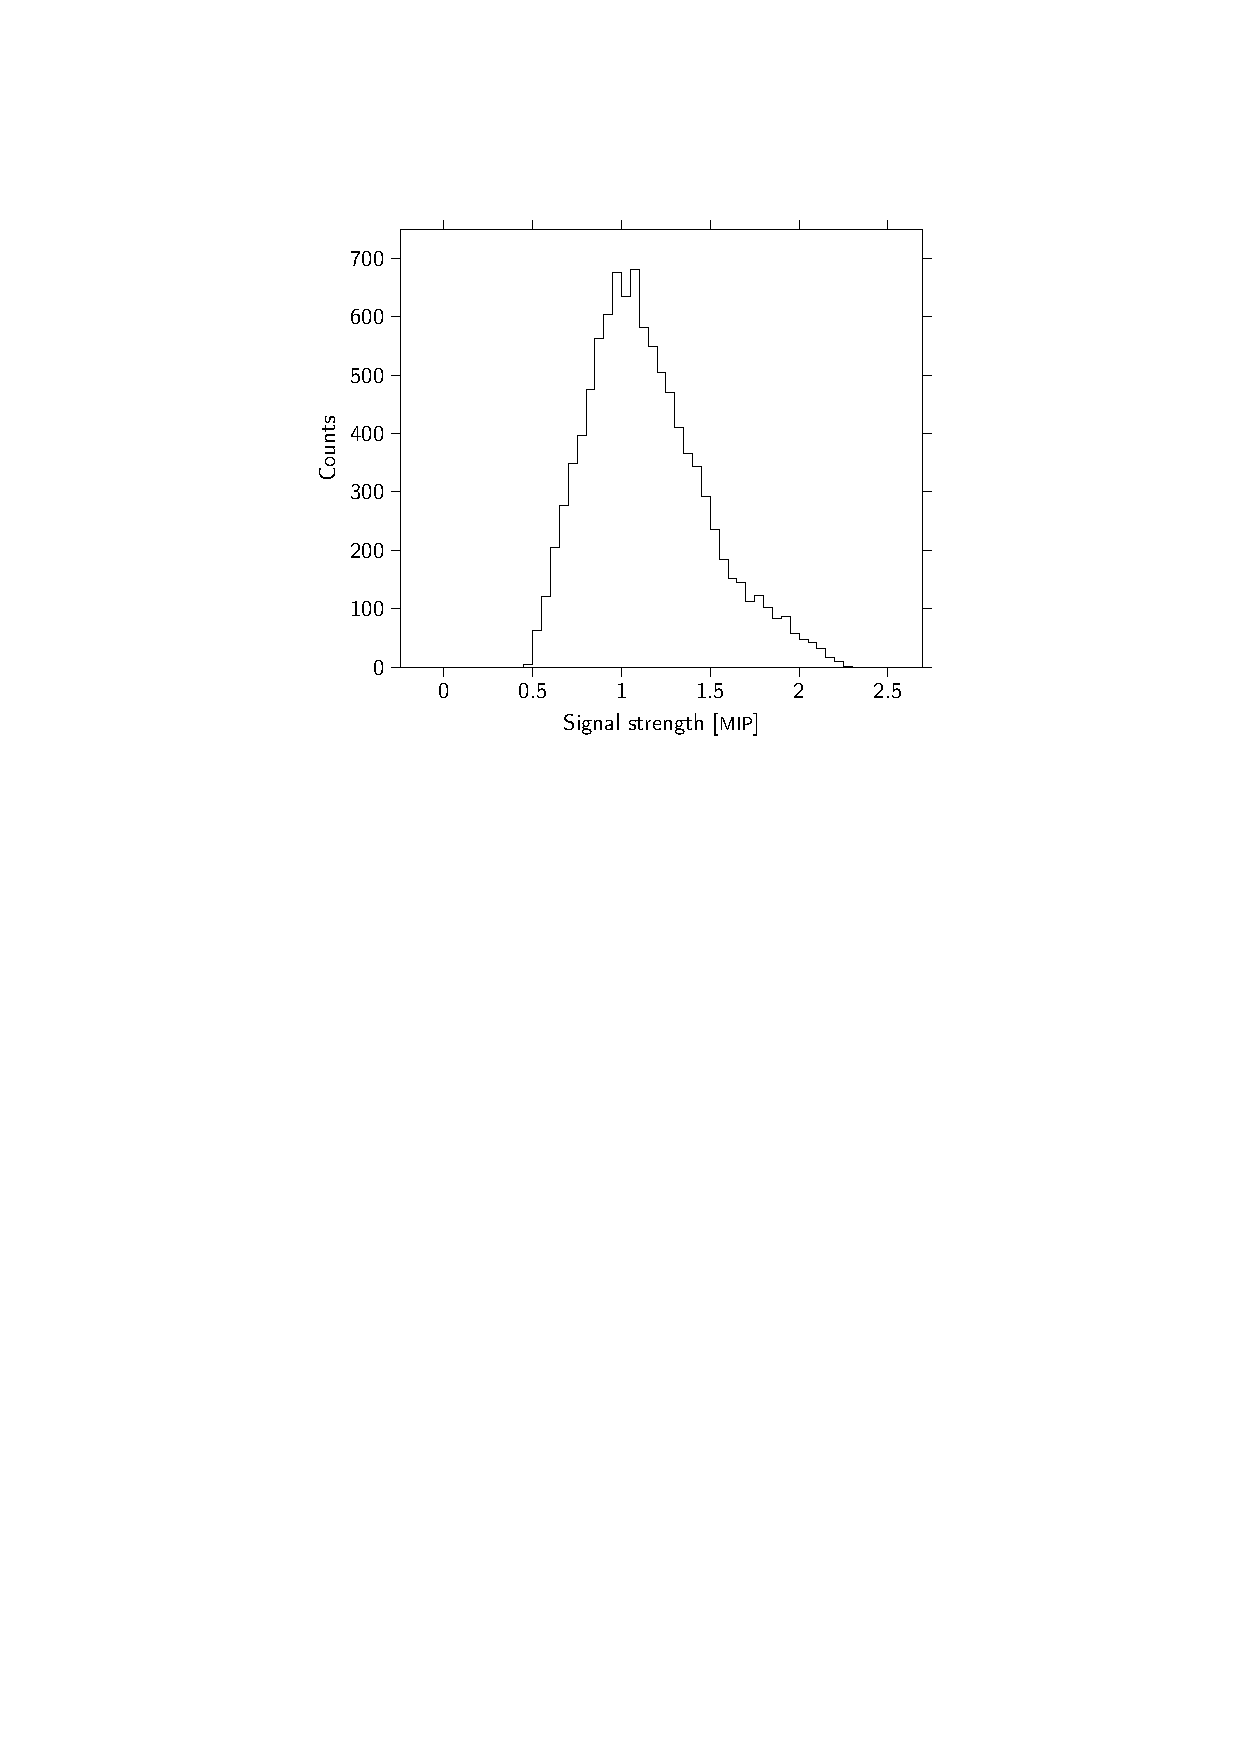
\includegraphics[width=0.6\textwidth]
                    {plots/station/signal_response}
    \caption{Signal response distribution a single lepton passing vertically through the scintillator detector. The transmission efficiency is statistically modelled. The effect of particle angle of incidence can be accounted for by scaling the x-axis with $\cos{\theta}^{-1}$.}
    \label{fig:signal_response}
\end{figure}

\begin{figure}
    \centering
    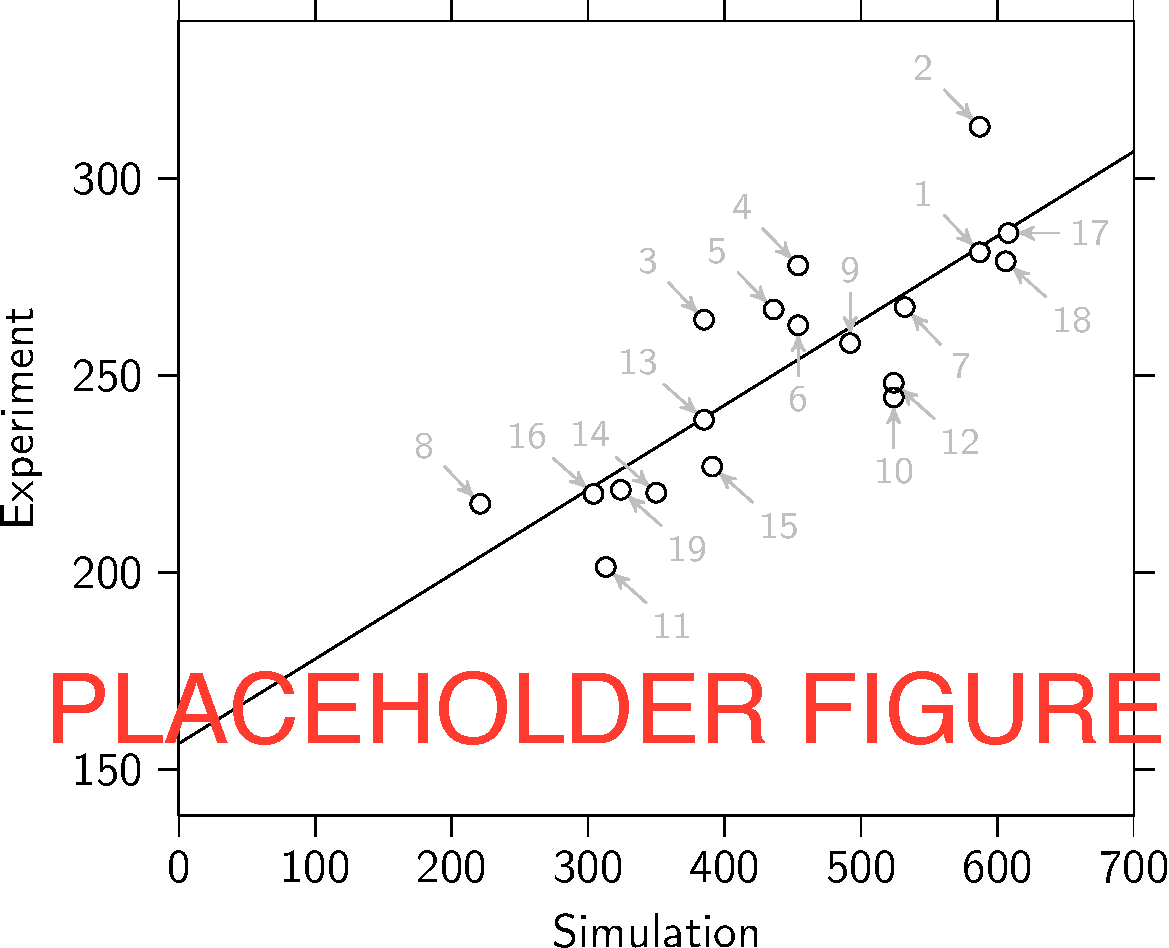
\includegraphics{plots/station/scintilator_transmission_compared}
    \caption{Correlation between the transmission efficiency for different positions in the scintillator between a real scintillator detector and the simulated one. The difference can be explained by the aluminium foil in which the detector is wrapped is not taken into account in the simulation. Moreover, some of the positions are in locations where the simulation predicts a significant gradient. [todo; use simulation which does account for Alu foil.]}
    \label{fig:scintilator_transmission_compared}
\end{figure}

Also the travel time of the photons to the \pmt varies depending on the location of emission and the emission direction. In \cref{fig:transport_time} the distribution of transport times is shown, the time is the arrival time when enough photons have reached the \pmt to produce a strong enough signal.

\begin{figure}
    \centering
    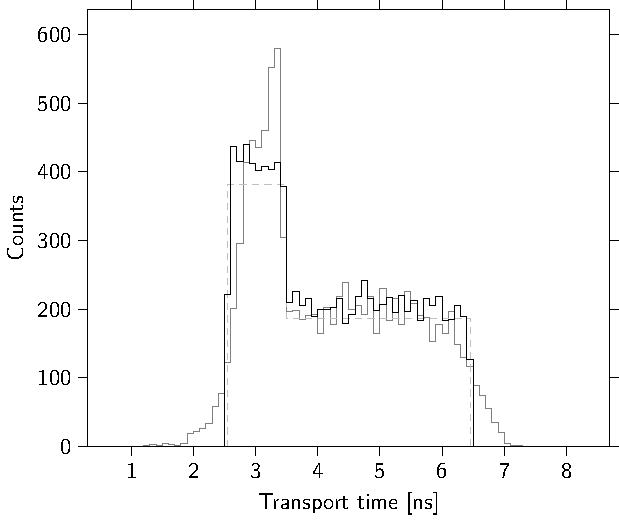
\includegraphics[width=0.6\textwidth]
                    {plots/station/transport_time}
    \caption{Transport time distribution for the scintillator detector. The scintillation light has to reach the \pmt from the point of impact, the travel time depends on the impact location in the scintillator, this is the overall distribution.}
    \label{fig:transport_time}
\end{figure}

The signals detected by the \pmt do not know where in the scintillator a particle hit, so these distributions add to the uncertainties of the measured quantities (signal strength and arrival time).


\subsection{Photomultiplier tubes}

% How PMT works
The photomultiplier tube has a front window with a photocathode. When this is hit by a photon an electron can be knocked free, due to the photoelectric effect. The probability that this happens is called the quantum efficiency, which is \SI{25}{\percent} for the scintillator light. The electron is then pulled along electric field lines which direct it to a dynode. The electron will cause multiple electrons to be emitted from the dynode, these electrons are then pulled to the next dynode, which has a higher positive potential. Each electron impacting the next dynode will cause the release of more electrons, which are accelerated towards the following dynode, and so on. At the end the electrons fall on the anode which is connected to the readout. This is shown in \cref{fig:pmt_schematic}.

\begin{figure}
    \centering
    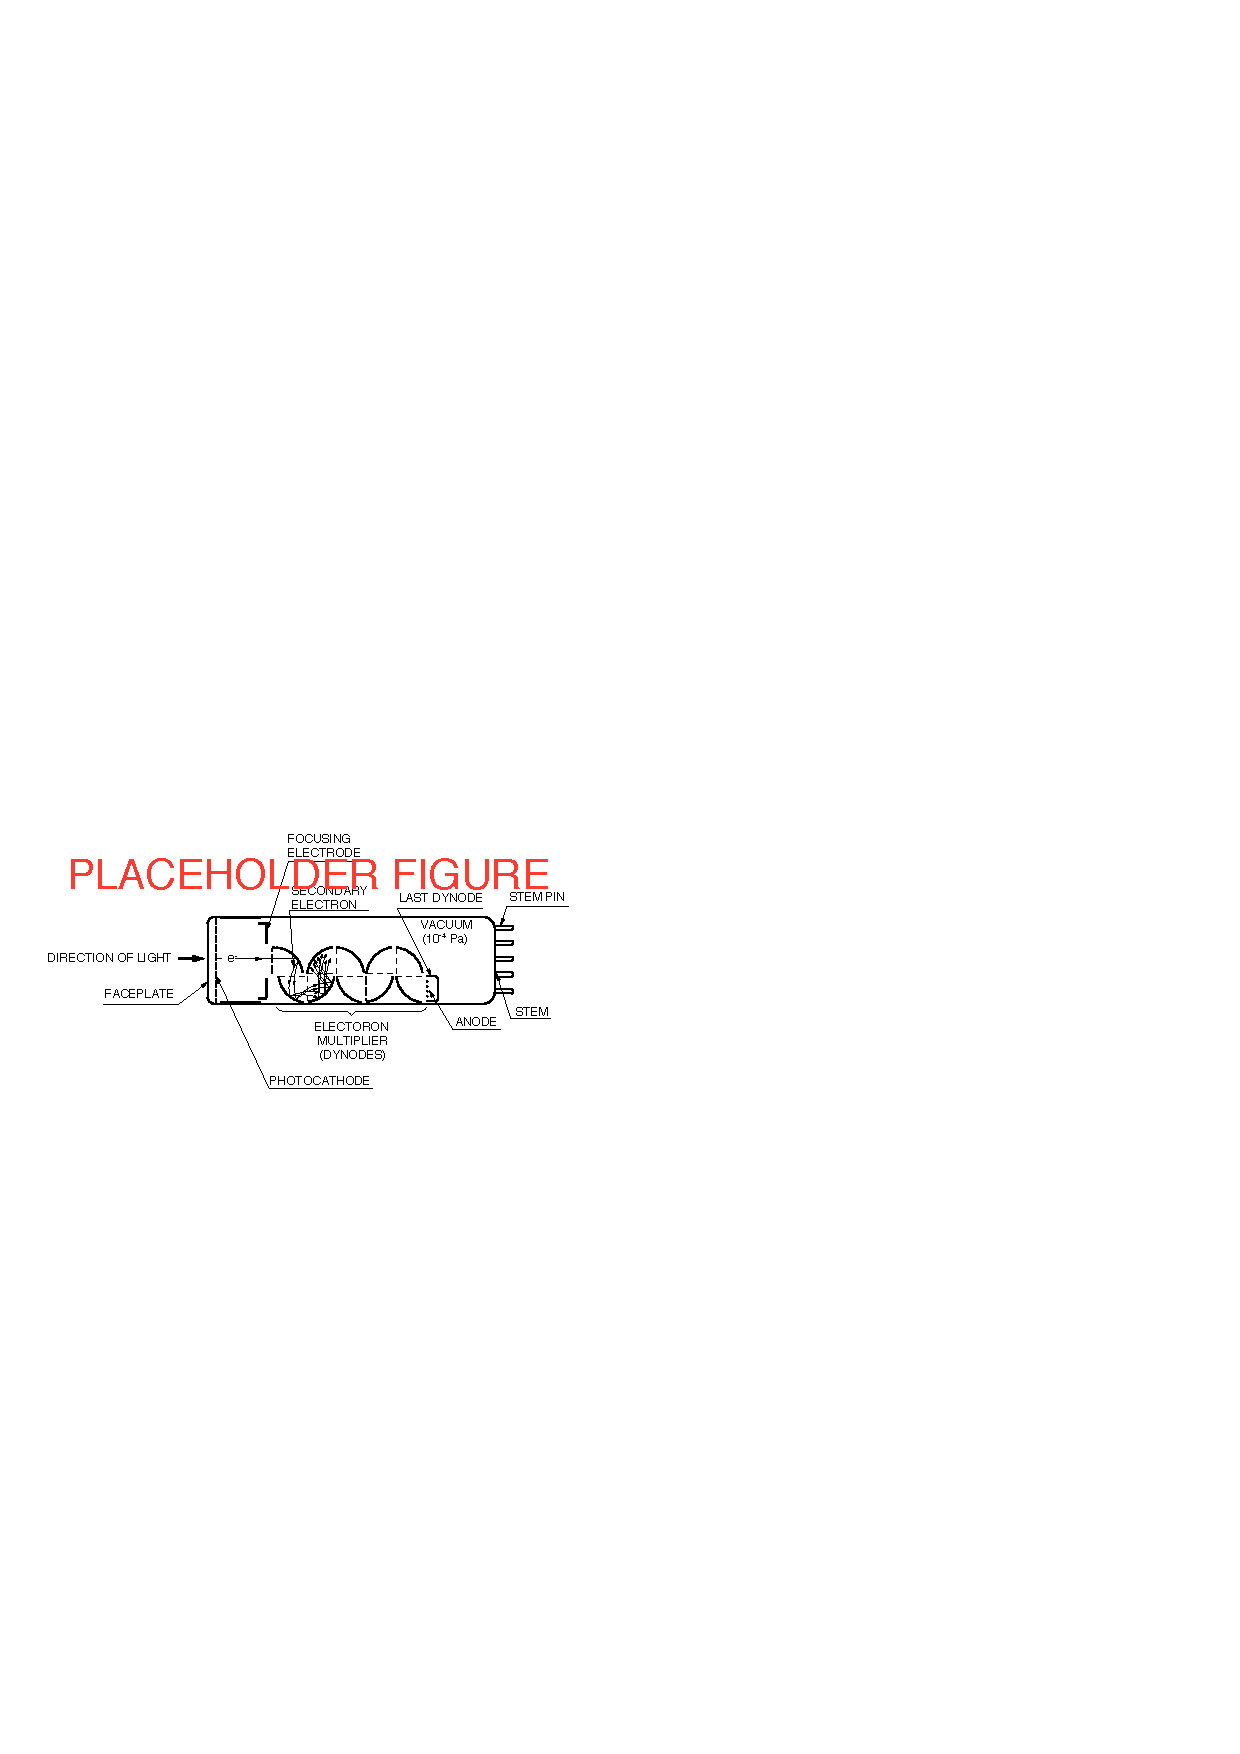
\includegraphics[width=0.6\textwidth]
                    {plots/station/pmt_schematic}
    \caption{Schematic crosssection of a \pmt.}
    \label{fig:pmt_schematic}
\end{figure}

% PMT gain, fluctuations in gain..
The \pmts which are used have 11 dynodes, this number affects the gain of the \pmt. If each electron causes \num{3} electrons to be released from a dynode then every electron falling on the first dynode will result in $3^11$ electrons at the anode. The number of electrons emitted by a dynode for each electron that falls on it may vary. This results in a variation in the output signal for each single photoelectron. This can vary  y a factor of 2, if for instance the first dynode emits either 2 or 4 electrons instead of 3. Typical variations in output, for the same number of created photoelectrons, are of the order of \SI{10}{\percent}. By changing the voltage on the dynodes the gain of the \pmt can be tuned, with a higher voltage resulting in a higher gain. The relation between gain and voltage is not linear \cite{hamamatsu2007handbook}.

% Signal strength is used for particle density, need to be able to distinguish between different number.
Both the scintillator and \pmt can handle multiple particles simultaneously and will produce correspondingly higher signal output. The integrated signal strength should be the sum of two individual particles. Given the width of the signal distribution for single particles given by the Landau distribution combined with the transport efficiency a single particle will in some cases (how often?) produce a signal equal or larger than the most probable signal strength of two particles. In \cref{fig:ph_histogram_contrib} an example of the expected pulse height histogram is shown including the contributions from gammas, and multiple leptons. The widths of the contributions are due to the particle inclination, Landau distribution, transmission efficiency, and \pmt variation. The first peak gives the most probable value (\mpv) for the pulse height of a single lepton. An approximation of the number of particles can be made by comparing a measured value to the \mpv. The position of the \mpv depends mostly on the transmission efficiency of the scintillator detector and the gain of the \pmt. By changing the voltage on the \pmt (i.e. on the dynodes) the position of the \mpv can be tuned. Ideally the \mpv is approximately \SI{150}{\mV}. If it is lower it is difficult to distinguish the lepton contribution from the gamma spectrum and the \mpv will be hard to determine. If the \mpv is at a much higher value the \pmt ages more quickly and the dynamic range [in number of particles..] will be reduced.

\begin{figure}
    \centering
    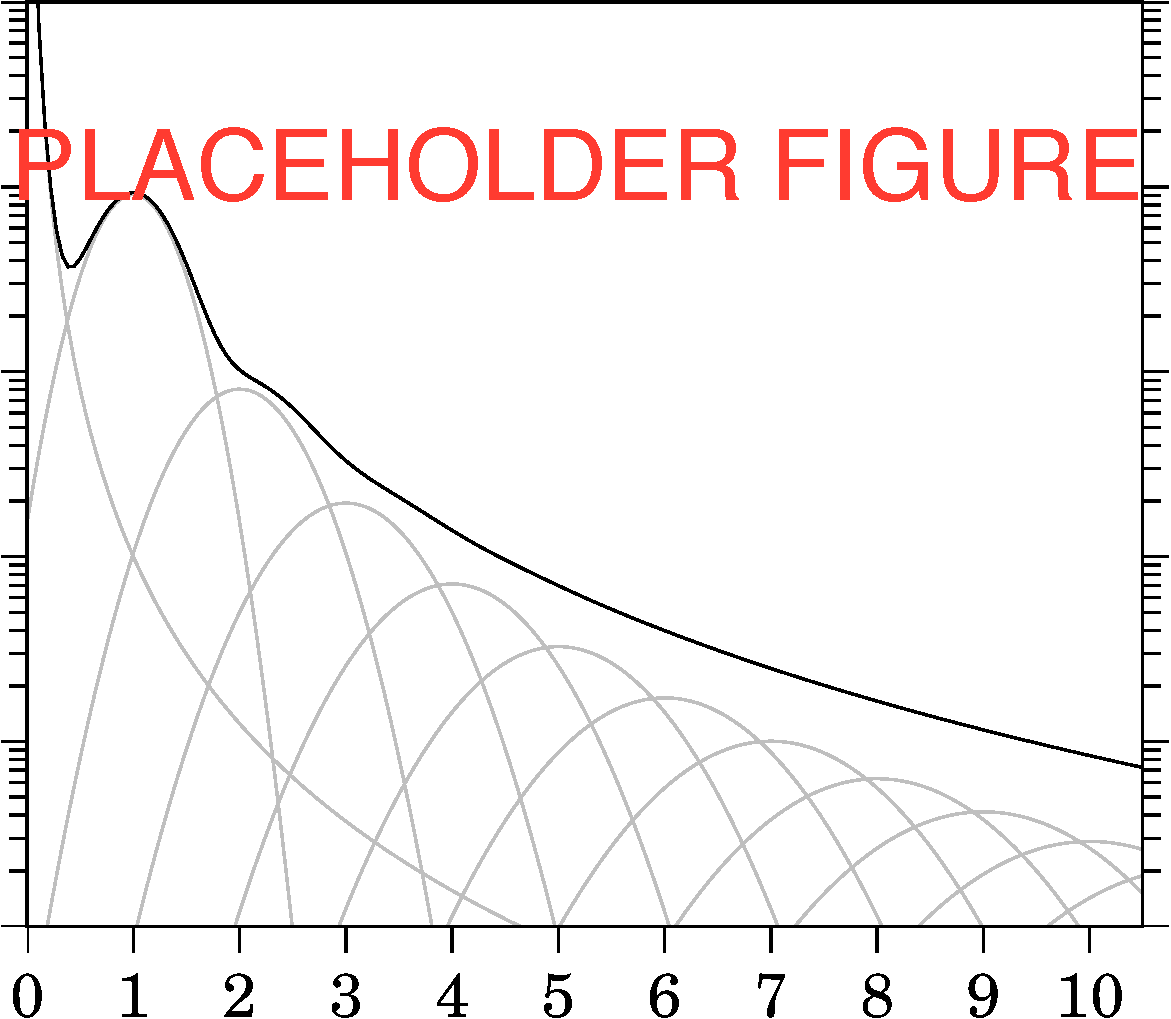
\includegraphics[width=0.6\textwidth]
                    {plots/station/ph_histogram_contrib}
    \caption{Overlap between pulse integral contributions from multiple mips in one event, the width of each contribution is due to Landau distribution and transport efficiency.}
    \label{fig:ph_histogram_contrib}
\end{figure}


\subsection{\pmt output linearity}
\label{sub:pmt_linearity}

% Why the PMTs are begin tested
An EAS may cause many particles to pass through a scintillator detector simultaneously. The response of the \pmt to different signal strengths needs to be investigated to determine the accuracy with which the number of particles can be reconstructed. Ideally the output of the \pmt grows linearly with the number of photons impacting its photocathode. Large signals from the \pmt, capable of saturating the readout \adcs, are expected to occur dozens of times a day. However, in the data we find that some \pmts never produce such large signals. It appears that the output is compressed at high values. Calibration tests have been performed on several \pmts to test their output given a known input signal.

% LED test setup
A setup has been created to test the linearity of \pmts using LED light flashes. A bundle of 24 optical fibers, each connected to a LED, are fed into a cap which directs the light at the photocathode of a \pmt. The LEDs can be triggered simultaneously to produce a short (\SI{20}{\ns}) pulse. This is similar to a pulse generator, but with light pulses. The intensity of light produced on the \pmt by a single fiber is comparable to one or two \mip in a scintillator detector. The \pmt pulse intensity typically fluctuates up to \SI{50}{\percent}. Taking the average over hundreds of pulses gives a very stable result.

\begin{figure}
    \centering
    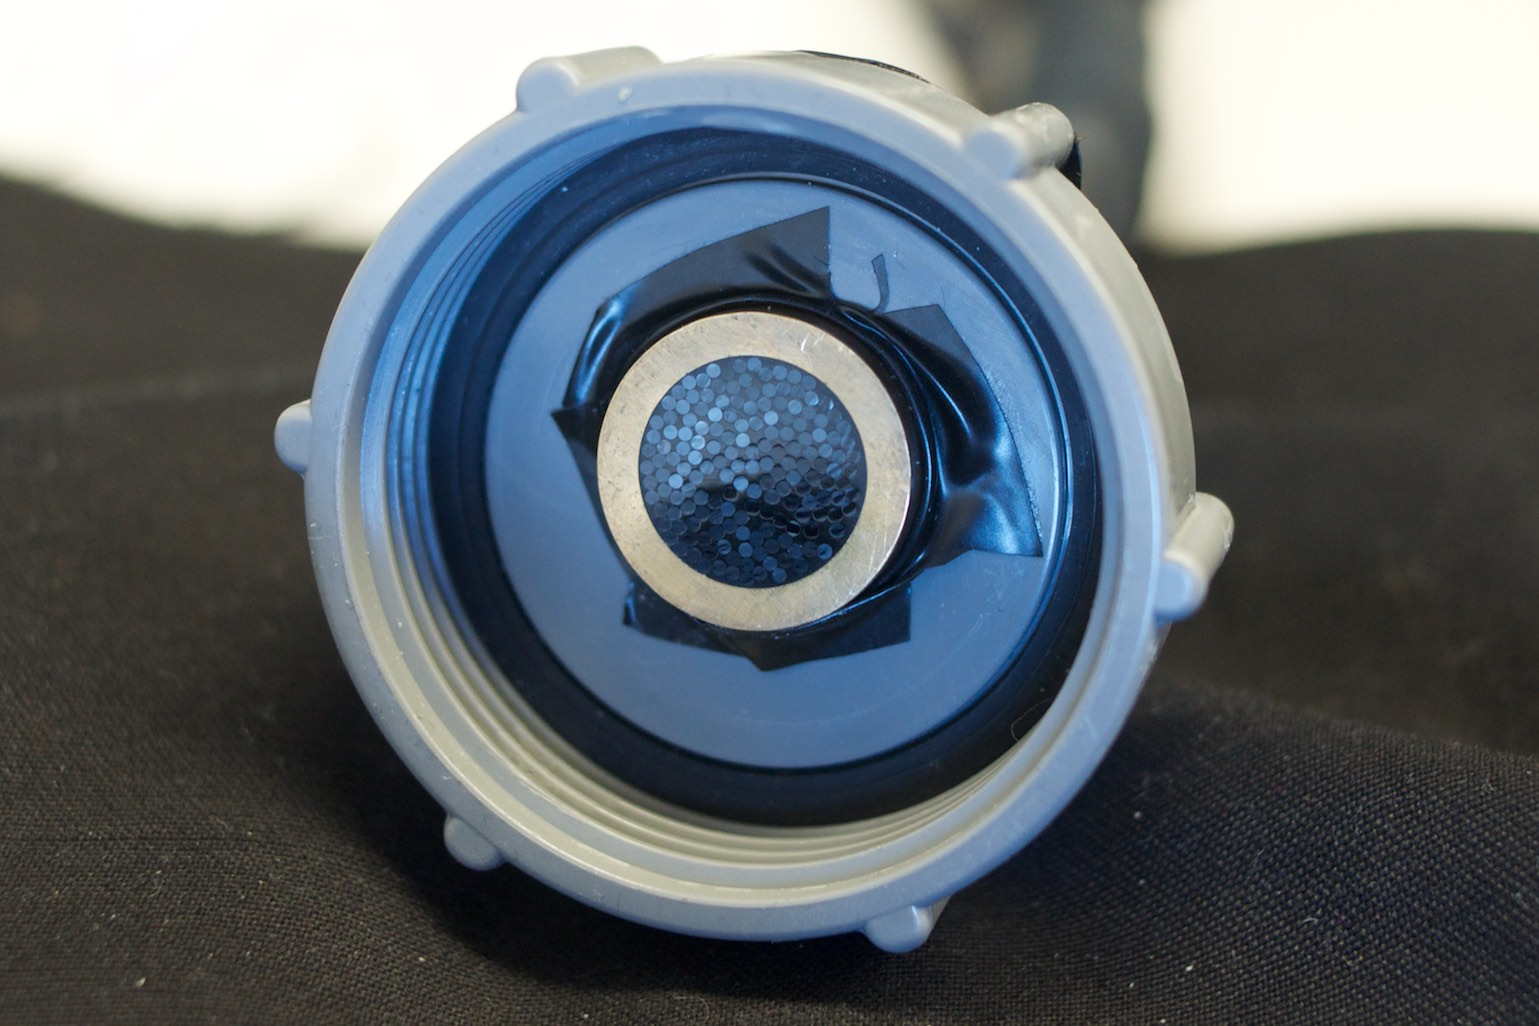
\includegraphics[width=0.45\linewidth]{plots/station/ARN_085351.jpg}
    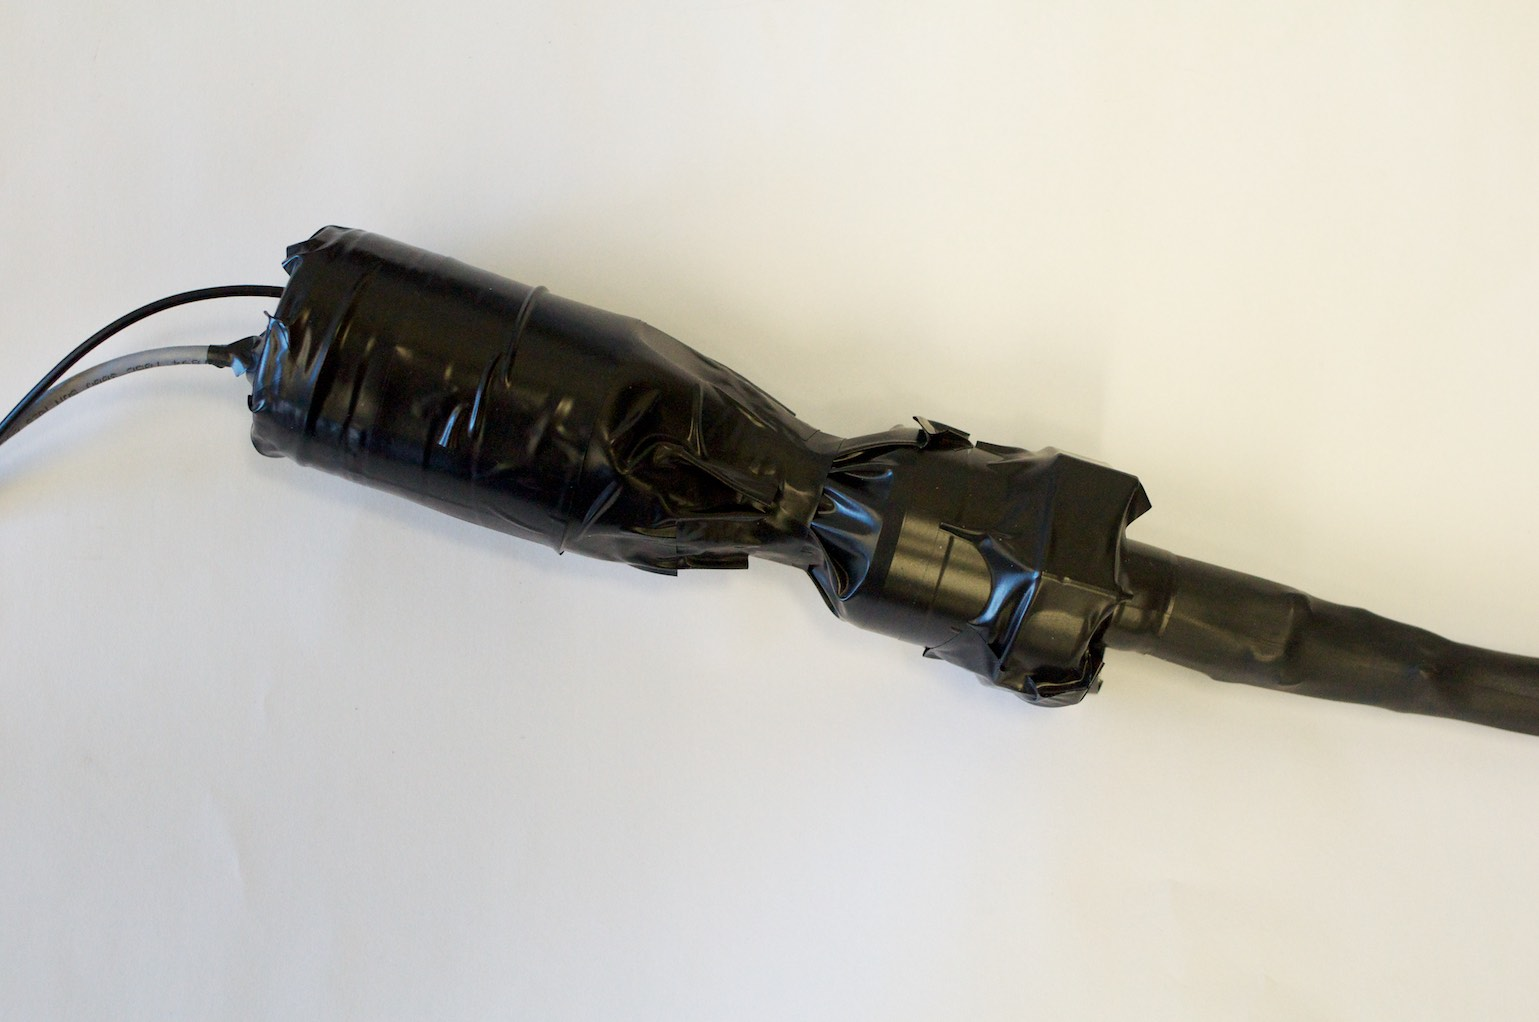
\includegraphics[width=0.45\linewidth]{plots/station/ARN_085349.jpg}
    \caption{Here the setup for the \pmt tests is shown. The first photo shows the fibers in the bundle. The second photo shows the bundle connected to a \nikhef \pmt, wrapped light tight with tape.}
    \label{fig:pmt_test_setup}
\end{figure}

% Test calibration
The mean intensity of the individual fibers is not equal. For each \pmt the mean intensity of each individual fiber is determined. This is done by turning off the other fibers. This makes it possible to determine the input signal when multiple fibers are connected, i.e. the sum of the individual contributions. Possible time delays between the pulses might make the resulting pulses wider instead of higher, so not only the pulse height is examined but also the pulse integral. Any subset of the 24 fibers can be used simultaneously. Signals with an expected \pmt output pulse height over \SI{5}{\volt} are possible with the full bundle of fibers, with the \pmt at normal operating voltage.

An oscilloscope is used to readout the \pmt signal. This allows for easy averaging of multiple signals and to readout signals larger than the \SI{2}{\volt} limit of the \hisparc electronics. The oscilloscope measures the signal's pulse height and integral.

% PMT test results
In \cref{fig:linearity_pmts} the results of two \pmt tests are shown. The \senstech \pmt starts to deviate from the straight line before the measured pulse height reaches \SI{1}{\volt}. With increased signal input it just barely reaches \SI{2}{\volt}. The \nikhef \pmt on the other hand is linear over the entire range that was measured. Larger input signals were not possible with the used setup, so it is unclear at what input the \nikhef \pmt will be unable to keep the output linear with the input.

% Fitting the data
The non-linear data can be fitted by an equation described in \cite{icecube2010pmt}. However, the parameters are very correlated and are not always able to accurately fit the data, this is especially the case for test data discussed later in \cref{sec:kascade_density}. A different phenomenological model has been devised, shown in \ref{eq:lin_circ_lin}. The model (on log-log axes) consists of two linear parts with different slopes ($a_1$ and $a_2$) and y-intercepts ($b_1$ and $b_2$), which are joined by a circle segment. For the first line the slope $a_1$ is fixed to 1 and the y-intercept $b_1$ to 0. The two linear components are tangent to the circle whose radius $r$ is also a free parameter. The final relation is described by
%
\begin{equation}
\label{eq:lin_circ_lin}
    \log y =
    \begin{cases}
        a_1 \log x + b_1,                     & \text{if $x \leq x_1$}.\\
        y_c \pm \sqrt{r^2 - \left(\log x - x_c\right)^2}, & \text{if $x_1 < x < x_2$}.\\
        a_2 \log x + b_2,                     & \text{if $x \geq x_2$}.
    \end{cases}
\end{equation}
%
Here $x$ is the recorded output and $y$ the expected output [TODO: fix dimensions of these quantities, different depending on what is fitted, so dimensionless preferable, but also fix plot axes..]. The center of the circle ($x_c$, $y_c$) is found by computing the intersection between two lines which are parallel to the original lines but shifted by a distance $r$
%
\begin{equation}
    \begin{aligned}
    x_c &= \frac{b^{\parallel}_2 - b^{\parallel}_1}{a_1 - a_2} \ ,\\
    y_c &= a_1 x_c + b^{\parallel}_1 \ ,
    \end{aligned}
\end{equation}
%
here the y-intercepts ($b^{\parallel}_1$ and $b^{\parallel}_2$) of the parallel lines are, with $i \in \{1, 2\}$, defined as
%
\begin{equation}
    b^{\parallel}_i = b_i \mp r \sqrt{1 + a_i^2} \ .
\end{equation}
%
The intersection points ($x_1$, $x_2$) between the lines and circle segment can be found by defining lines perpendicular to the original lines and passing through the center of the circle. The intersection then becomes
%
\begin{equation}
    x_i = \frac{b^{\bot}_i - b_i}{a_i - a^{\bot}_i} \ ,
\end{equation}
%
where the slope and y-intercepts of the perpendicular lines are given by
%
\begin{equation}
    \begin{aligned}
    a^{\bot}_i &= -\frac{1}{a_i} \ ,\\
    b^{\bot}_i &= \left(a_i + \frac{1}{a_i}\right) x_c + b^{\parallel}_i \ .
    \end{aligned}
\end{equation}
%
The signs in the equation of the circle segment and the intercepts of the parallel lines depend on the slopes $a_1$ and $a_2$. If $a_1 > a_2$ use the upper signs, otherwise use the lower signs.

\begin{figure}
    \centering
    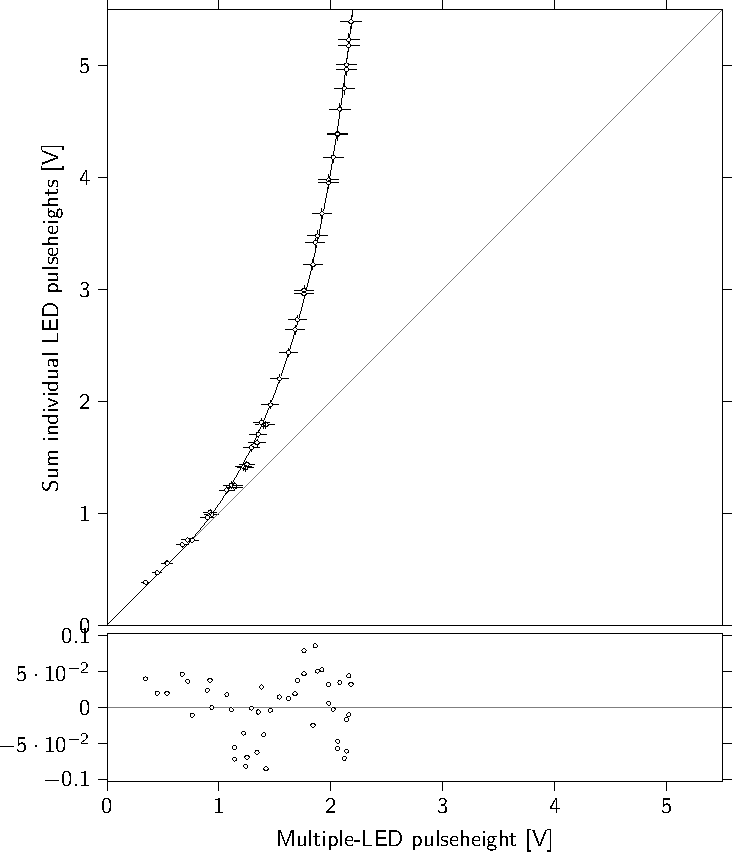
\includegraphics[width=0.7\linewidth]{plots/station/data_ph_senstech}
    \caption{Measurements of the pulse height linearity of \pmts. The dependence of the pulse height output on the input light intensity is shown. The input on the horizontal axis is scaled so that the inputs and outputs for the individual fibers are equal. The data points show the results from tests with the \senstech \pmt (closed circles) and the \nikhef \pmt (open circles). The black lines are fits to the data. [Todo: combine data from multiple tests in one plot]}
    \label{fig:linearity_pmts}
\end{figure}

The pulse height and pulse integral were both measured during the tests. The relation between these quantities is shown in \cref{fig:ph_pi_compared_nikhef_senstech} for the different \pmts. The relationship is linear for the \pmt with the \nikhef power supply, and non-linear for the others. The curve starts steeper for the \senstech \pmt, which means the output pulses are a bit slimmer (height versus width ratio).

\begin{figure}
    \centering
    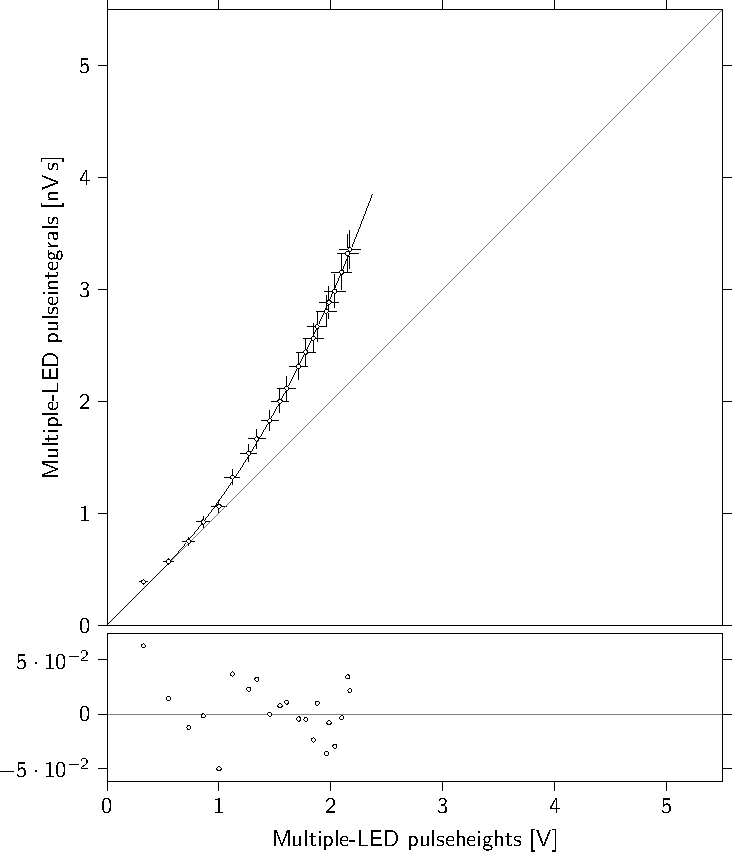
\includegraphics[width=0.7\linewidth]
                    {plots/station/data_piph_senstech_integral}
    \caption{Measurements of the pulse height versus pulse integral. The data points show the results for the \senstech \pmt (closed circles) and the \nikhef \pmt (open circles). The last data point for the \nikhef \pmt has an unexplained offset, possibly due to a bad measurement.}
    \label{fig:ph_pi_compared_nikhef_senstech}
\end{figure}

% Compare pulseheight and intergral for real data
In \cref{fig:ph_pi_503} cosmic-ray data is shown comparing the pulse height and integral of two scintillator detectors, one with a \nikhef \pmt, the other width a \senstech \pmt. The \senstech \pmt clearly does not utilize the full dynamic range of the readout, while the other does. The pulse integral continues to grow for both, even when the \nikhef \pmt saturates the readout. This is explained by the pulse becoming wider at its base. The pulse integral grows slower when some of the samples in the pulse are saturated. The non-linearity causes the higher pulseheights to be condensed, the contributions to the pulseheights would look like \cref{fig:ph_histogram_contrib_nonlin}.

\begin{figure}
    \centering
    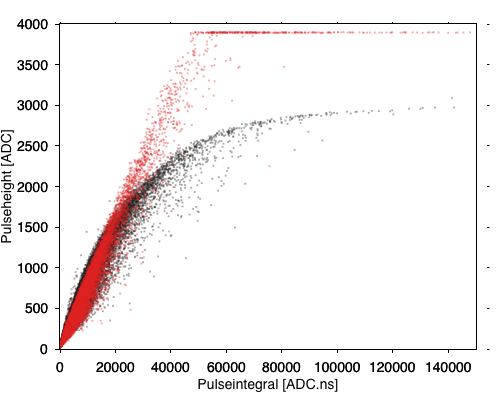
\includegraphics[width=0.7\textwidth]{plots/station/ph_pi_503.png}
    \caption{Measured pulse height versus pulse integral from a scintillator detector data. The data is from detector 1 and 2 from station 503. Detector 1 (black) uses a \senstech \pmt, detector 2 (red) uses a \nikhef \pmt.}
    \label{fig:ph_pi_503}
\end{figure}

\begin{figure}
    \centering
    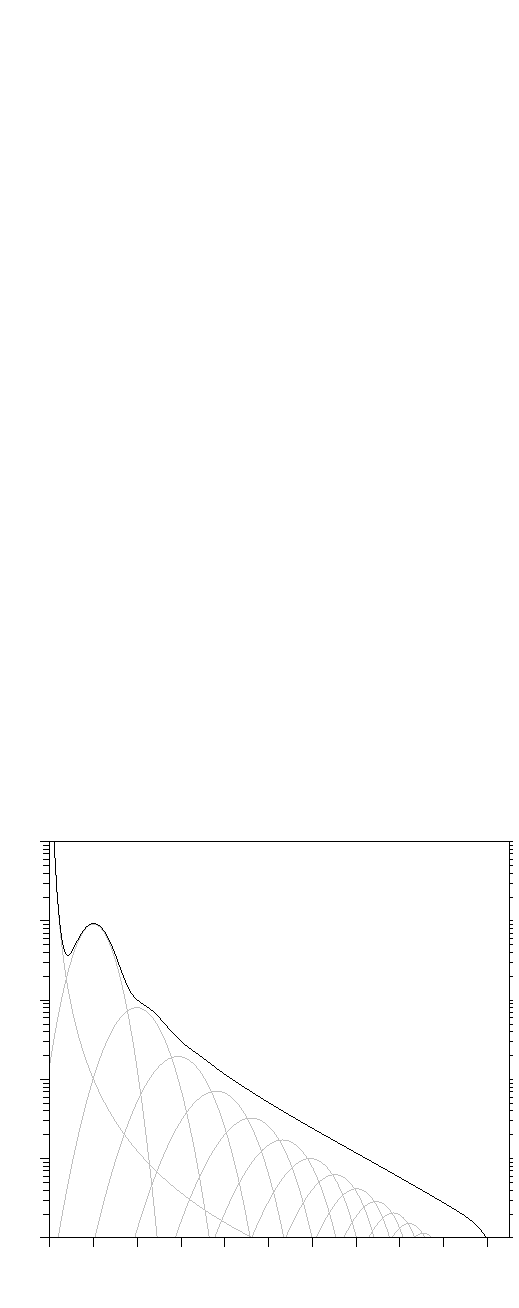
\includegraphics[width=0.6\textwidth]
                    {plots/station/ph_histogram_contrib_nonlin}
    \caption{Pulseheight histogram as in \cref{fig:ph_histogram_contrib}, but with a non-linear \pmt, causing the end to be condensed. [todo: fix area count]}
    \label{fig:ph_histogram_contrib_nonlin}
\end{figure}

% Applying corrections to data
For each \senstech \pmt a different correction needs to be applied to the detected signals. Unfortunately, almost no \pmts have been calibrated using the LED setup. It is impractical to do so for all already installed scintillator stations. Fortunately the \pmts are relatively linear up to \SI{1}{\volt}. Measured cosmic data does provide some insight into the non linearity. Partial information may be obtained via the pulse height and integral relation, however, those are not independent measurements.

% Testing new PMTs
Since April 2014 the new \nikhef \pmts are first tested in the LED setup using a single fiber to ensure it works properly. The test finds the voltage at which the output has a pulse height around \SI{340}{\milli\volt}. This pulse height value requires a voltage close to the normal operational voltage of \pmts on a scintillator detector. The current of the \pmt is also checked, high currents can indicate failing \pmts. The linearity tests are currently to cumbersome to perform for each \pmt. Moreover, most new \pmts use the \nikhef power supply and should not require calibration.


\subsection{Temperature in the skibox}

The specifications of the scintillator and \pmt indicate that their efficiency depends lightly on their temperature \cite{sgc2011bc408,et2010pmt}. The pulse height of signals determine wether they cross signal thresholds used for triggering, increased efficiency would cause more triggers, while with reduced efficiency some events may be missed. The change in efficiency also affects the \mpv. The effect of temperature on the \mpv will be examined.

For short periods temperature probes have been placed inside the skibox and attached to the \pmt of a scintillator detector to accurately measure the local temperature. In \cref{fig:temperature_timeline} the values from these sensors for a month can be seen. The daily (day and night) fluctuations can clearly be seen. The skibox and \pmt temperatures clearly rise above the outside temperature. This is mostly due to the absorption of solar radiation by the skibox, and the heat generated by the \pmt itself. There is little to no air flow inside the skibox. On sunny days the temperatures in the skibox rise a lot higher than the outside temperature. Using solar radiation data the outside temperature can be corrected to accurately describe the skibox temperature (see \cite[Figure 7.7]{devries2012weather}).

\begin{figure}
    \centering
    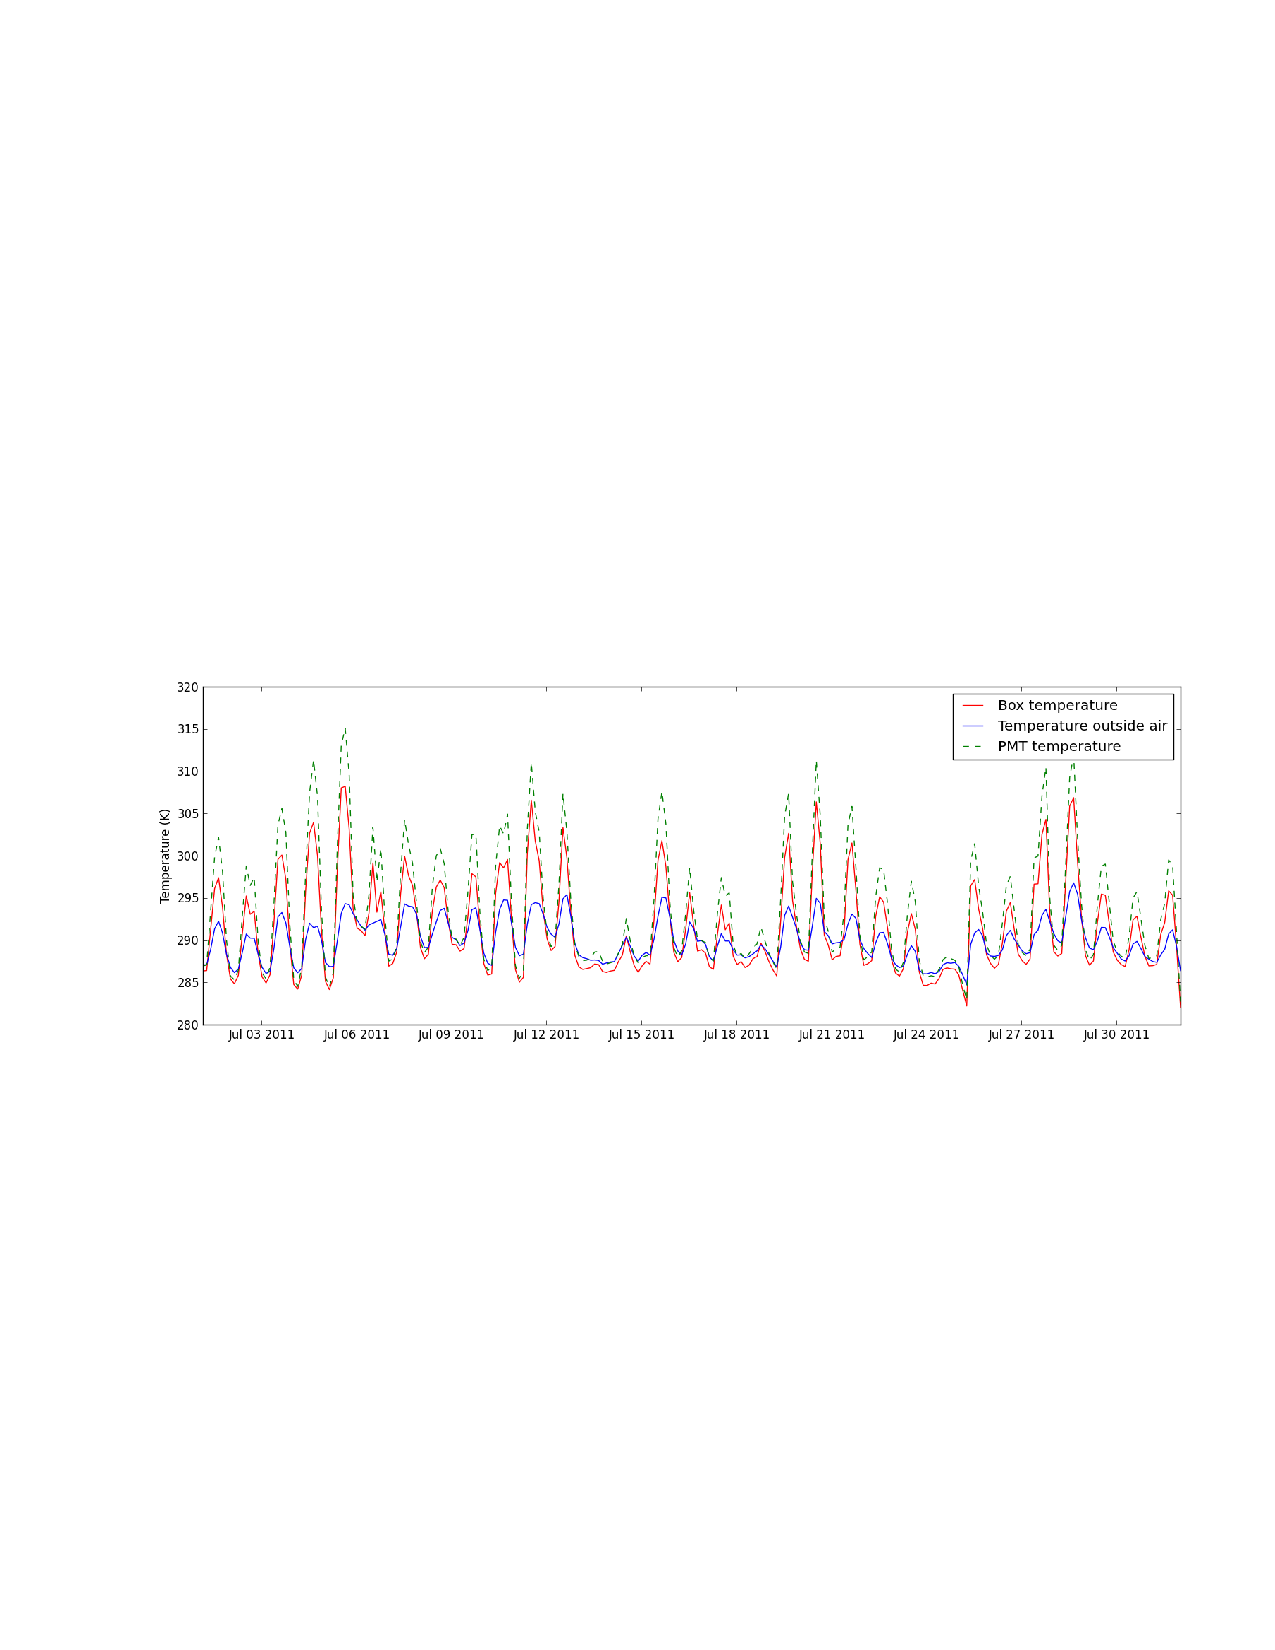
\includegraphics[width=\linewidth]{plots/station/temperature_timeline}
    \caption{Measured temperatures over time from several different sensors. A temperature probe was placed inside a \hisparc detector skibox (blue). Another sensor was attached to the \pmt of the detector (green). The weather station connected to the \hisparc station also has a temperature sensor.}
    \label{fig:temperature_timeline}
\end{figure}

A day of data is enough to accurately determine the average \mpv for that day. However, daily temperature fluctuation are large enough that when the days is broken into smaller pieces different values for the \mpv are found \cite{bartels2012mpv}. In \cref{fig:mpv_temperature} the reconstructed \mpv (for 4 hour intervals) is set against the \pmt temperature. The spread around the fitted line is partially caused by the temperature gradient in the periods for which the \mpv is determined. The correlation agrees reasonably with the specifications of the \pmt. The specification states the gain of the \pmt changes by \SI{0.5}{\percent\per\degreeCelsius}. It does not make clear wether the efficiency increases or decreases with changing temperature, nor at which temperature it is most efficient. From these measurements it seems the gain decreases with increasing temperature. The scintillator should be \SI{100}{\percent} effective up to \SI{20}{\degreeCelsius} above which it reduces with \SI{0.125}{\percent\per\degreeCelsius}. This is but a small contribution to the reduction of the \mpv. The found gradient of \SI{-0.81}{\adc\per\degreeCelsius} in the range \SIrange{200}{170}{\adc} is \SI{0.44}{\percent\per\degreeCelsius}, in close agreement with the specification. The same effect was found in \cite[Section 3.6]{lio2011}. However, in \cite[Section 3.5]{lio2010} experiments were performed that showed a positive correlation between temperature and the \mpv of a \pmt. Note that a different type of \pmt was used in those tests.

\begin{figure}
    \centering
    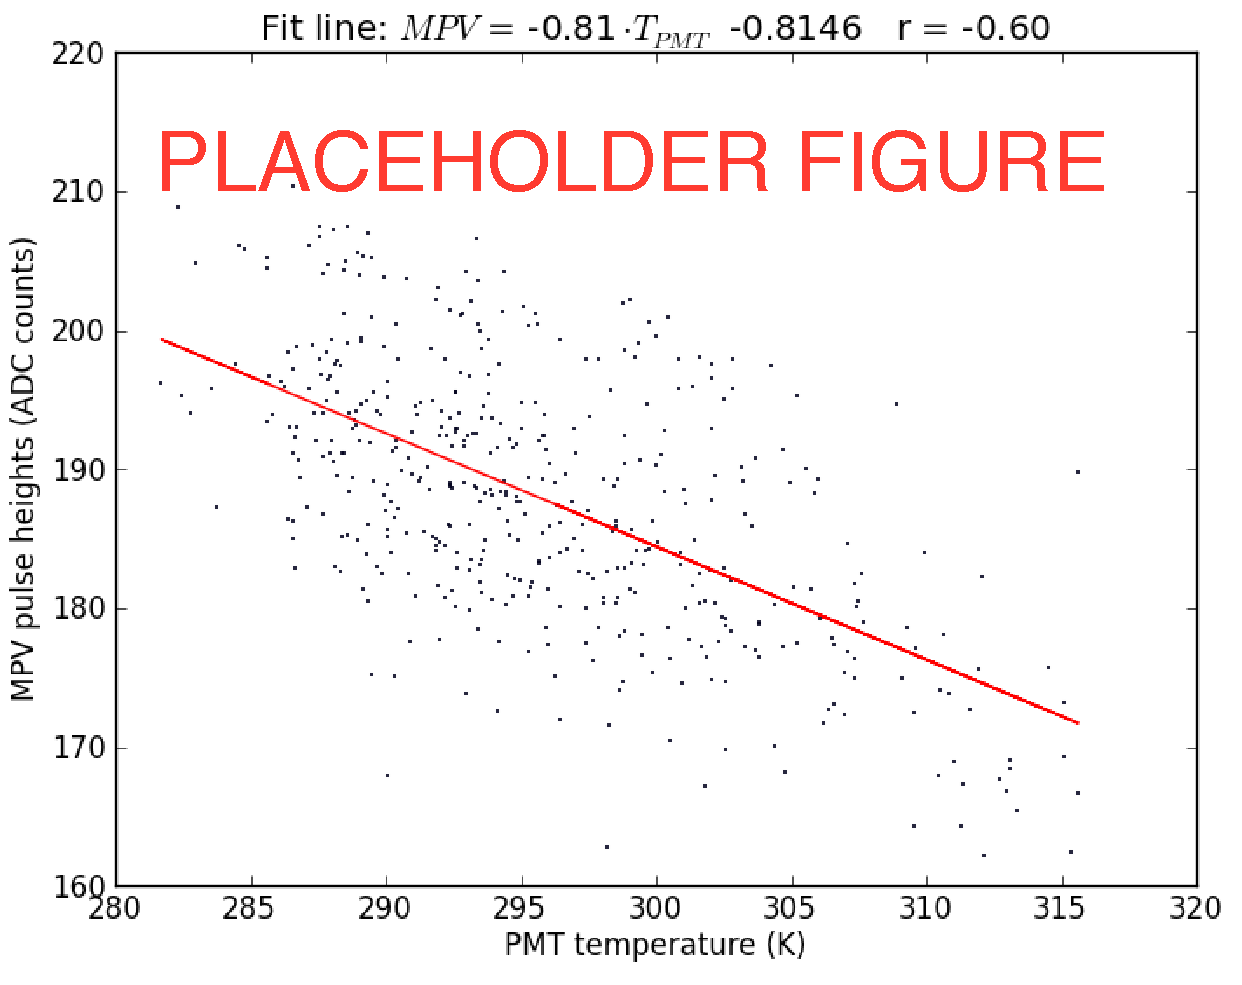
\includegraphics[width=0.7\linewidth]{plots/station/mpv_temperature}
    \caption{Here we can see the correlation between the measured temperature and the \mpv of the pulse heights. The red line is a linear fit to get the slope of the correlation.}
    \label{fig:mpv_temperature}
\end{figure}

Weather station data is available to correct measurements for the change in efficiency. The correction can be done using the outside temperature and solar radiation. However, this is less accurate then when the exact \pmt temperature is known. Solar radiation depends on cloud cover, which may be very different from location to location depending on wind speed. Moreover, some detectors may be in the shade for parts of the day, this may mean differences of \SI{20}{\degreeCelsius} between the expected and actual temperature.


\section{\hisparc electronics}

% Impractical to connect detectors over long distances for online/realtime triggering.
The \hisparc electronics incorporates \pmt readout and control, triggering logic, a \gps module \cite{trimble2007resolutiont}, and a data connection to a PC. Each \hisparc electronics unit is capable of controlling and reading out two \pmts simultaneously and performing signal strength and coincidence triggering. The data acquisition in the electronics is steered by a field-programmable gate array (\fpga). The front of the electronics is shown in \cref{fig:hisparciii_front}.

\begin{figure}
    \centering
    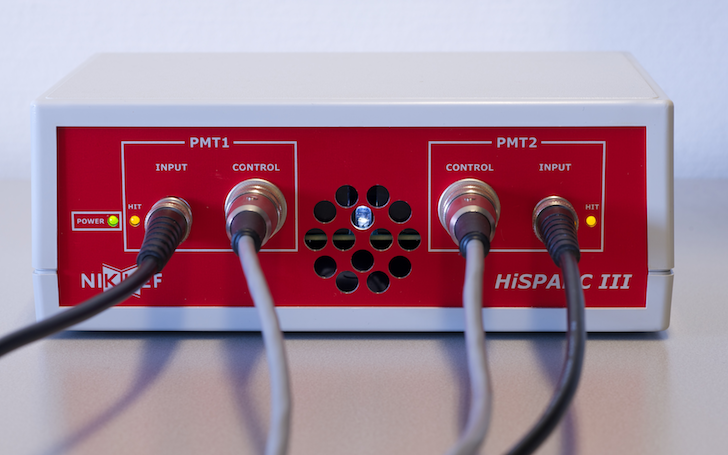
\includegraphics[width=0.6\textwidth]
                    {plots/station/hisparciii_front_power_hit_trigger.png}
    \caption{A powered \hisparc electronics with connected detectors. The orange LEDs next to the signal input activate when a signal in that channel is over the low thresholds. The center LED (white) indicates the occurrence of a trigger.}
    \label{fig:hisparciii_front}
\end{figure}

Two versions of the electronics are currently being used, versions II and III. Version III differs from II in having USB 2 (\SI{480}{\mega\bit\per\second}) instead of USB 1.1 (\SI{12}{\mega\bit\per\second}) connectors, slightly different \adcs, and an upgradable firmware over USB. The PC connected to the electronics contains software to send (configuration) and receive (data) messages to and from the \hisparc electronics. The message formats and their meaning are described in \cite{verkooijen2008firmware}, further description of the software running on the station PCs is described in [later chapter]. The scintillator detectors and \gps antenna \cite{trimble2015bullet} are connected to the electronics using \SI{30}{\meter} long cables.


\subsection{Signal readout}

The \hisparc electronics has two \adcs per channel, each \adc reads the \pmt signal at \SI{200}{\mega\hertz}. By interlacing the two \adcs a sampling frequency of \SI{400}{\mega\hertz} is achieved. These are 12-bits \adcs, allowing values between \SIrange{0}{4095}{\adc} and provide approximately \SI{2}{\volt} dynamic range. The two \adcs for one channel are calibrated to provide the same baseline and gain. The two electronics versions use a different type of \adc, with a slightly different dynamic range. The \si{\mV} to \si{\adc} conversion differs slightly, being \SI{0.57}{\adc\per\mV} (\hisparcii) and \SI{0.584}{\adc\per\mV} (\hisparciii). The baselines are set to \SI{200}{\adc} (\hisparcii) and \SI{30}{\adc} (\hisparciii). This results in an effective range of \SIrange{-2.222}{0.113}{\volt} (\hisparcii) and \SIrange{-2.374}{0.018}{\volt} (\hisparciii). In addition to the \adcs each channel has two comparators which record the time over threshold for a given threshold. The thresholds of the comparators can be configured over a large voltage range, but are by default set to \SI{-5}{\volt} and \SI{-10}{\volt}. In case of signals which saturate the \adcs the comparators provide additional information about the actual signal size. In \cref{fig:trace} an example readout of a pulse is shown. Subsequent signals from particles later in the shower front may be distinguished and the shower rise time can be examined.

\begin{figure}
    \centering
    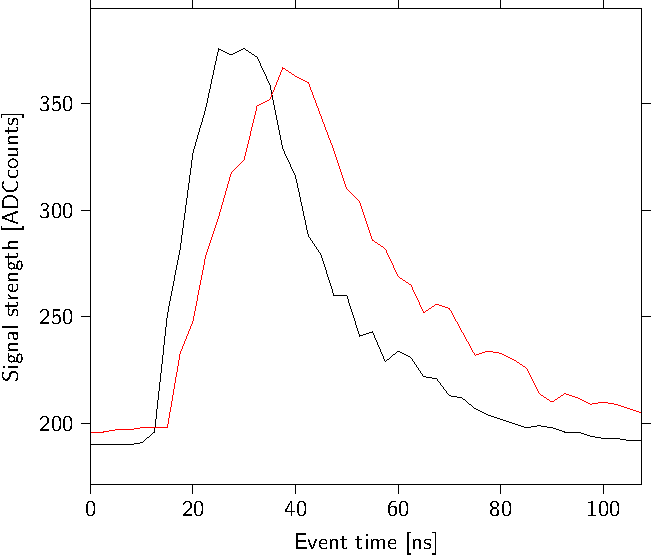
\includegraphics[width=0.6\textwidth]
                    {plots/station/trace_3501_1452556812_204602455}
    \caption{An example trace readout of two \pmts. The integrals of the signals are approximately the value of the \mpv. So most likely each scintillator detector detected a single lepton.}
    \label{fig:trace}
\end{figure}


\subsection{Comparators}

The non-linearity of the \pmt response described in [ref pmt lin section] means that many \pmts will never or hardly ever saturate the \adcs. The \hisparc electronics also includes two comparators per channel which determine if a signal reaches two higher thresholds (\SIrange{2}{10}{\volt}). These will remain unused with most stations, as they use the non-linear \pmts. For the new \pmts the comparators will be essential in signal reconstruction of high particle densities. However, the readout of the comparators was not implemented in the software until the end of 2015. So these will not be taken into further account in this thesis. Saturated pulses may still be reconstructed by fitting the non-saturated flanks of the pulses \cite[Section 3.5]{lio2011}. Double checking these fits with comparator data needs to be done first.


\subsection{\adc alignment}

In order to get consistent data both \adcs for each channel are aligned to have the same baseline and gain. \adcs remain accurate when they have a constant temperature. When \hisparc electronics are first connected the temperature will likely be below operating temperature. When calibration is performed immediately after powering the electronics it may drift from proper calibration as it continues to operate [how much drift?]. An offline/software based Mean Filter [ref to later section] in the software is capable of smoothing any remaining offsets in the combined signal. Note that this filter occurs after the trigger, so the trigger sees the unfiltered values. An example of misaligned traces is shown in \cref{fig:adc_alignment}.

\begin{figure}
    \centering
    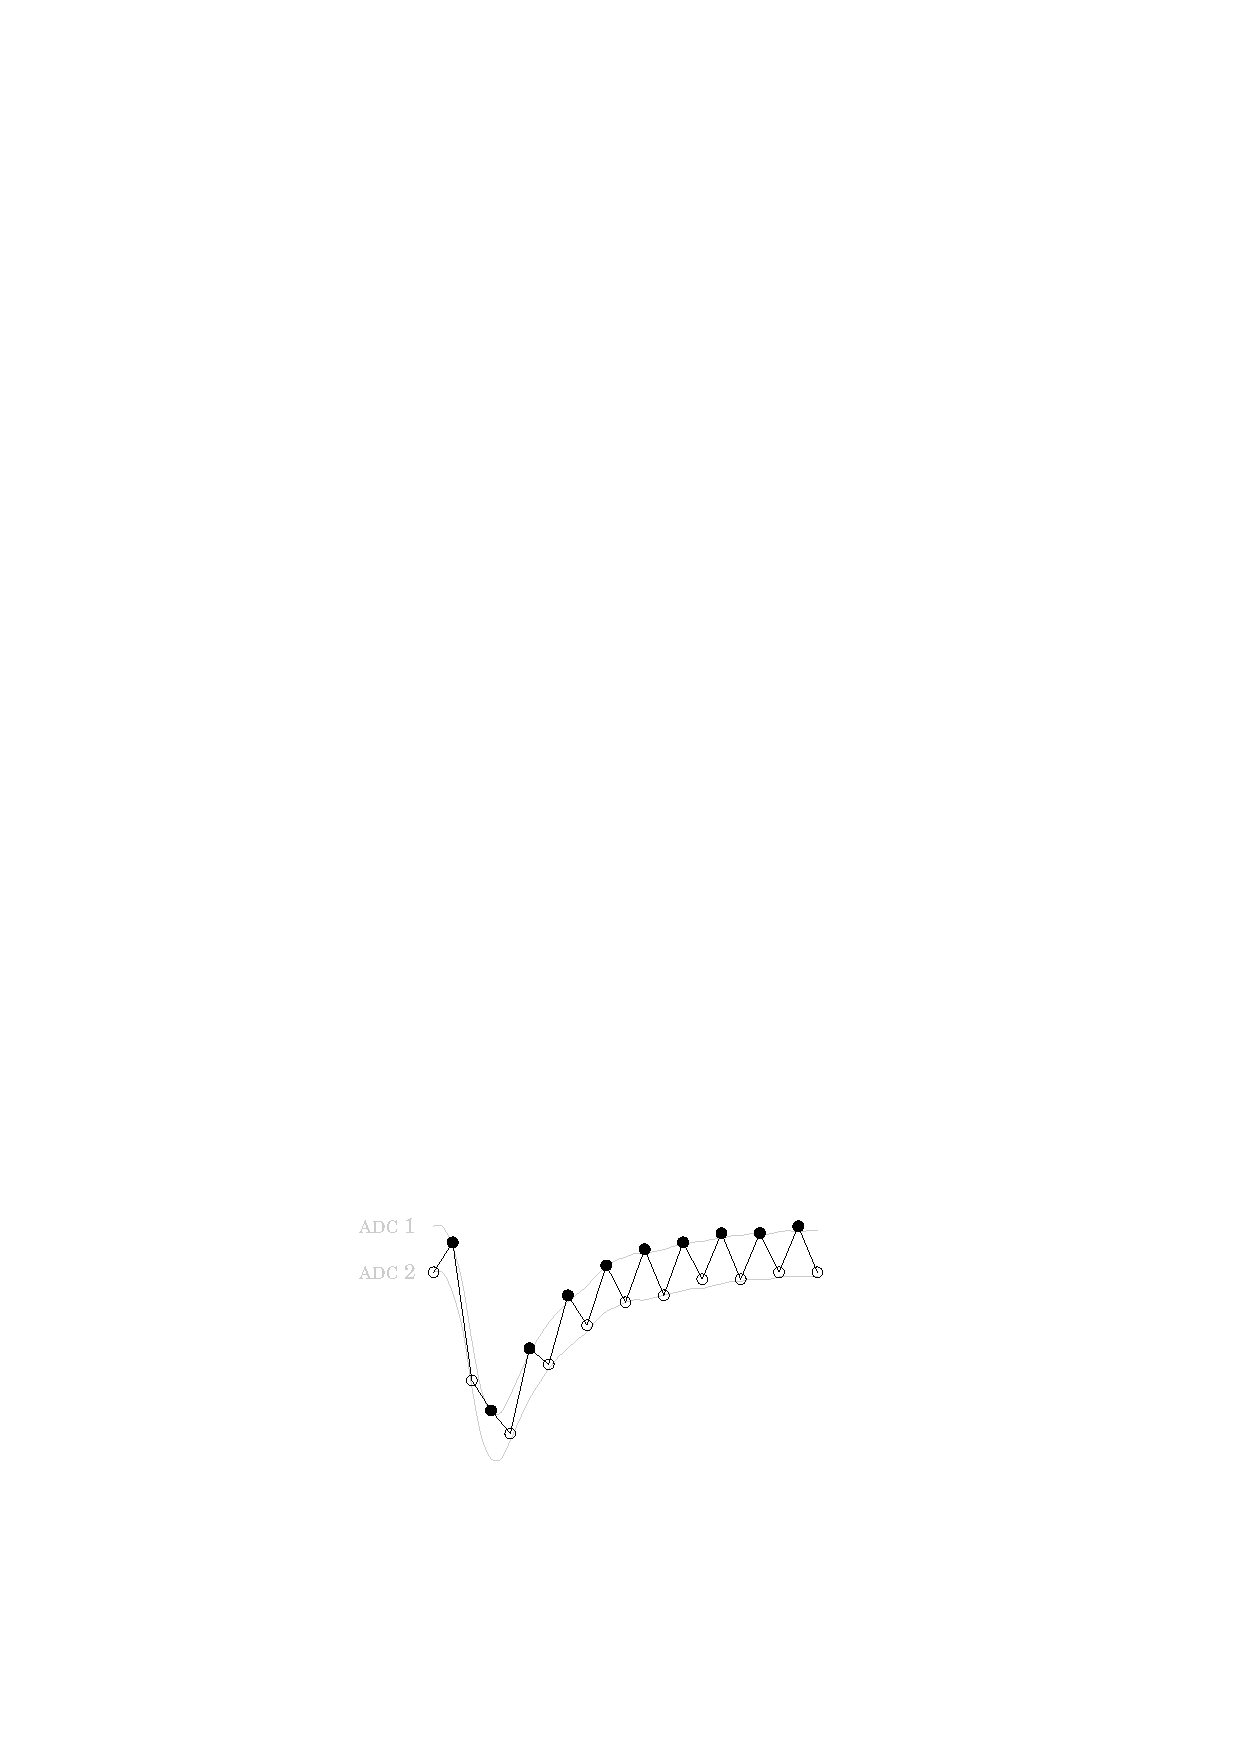
\includegraphics{plots/station/adc_alignment}
    \caption{Signals are read by two \adcs alternatively (open and closed circles). When the \adcs are not properly aligned they return different results for the same input.}
    \label{fig:adc_alignment}
\end{figure}


\subsection{Trigger thresholds and windows}

The \pmt signals are continually read out, the resulting \adc values for each channel are compared to two thresholds; a low and high threshold. These thresholds can be set for each channel individually. Usually they are set equally for all channels in a station, and the default setting is \SI{-30}{\milli\volt} (low) and \SI{-70}{\milli\volt} (high). These correspond to \SI{53}{\adc} (\hisparcii) or \SI{50}{\adc} (\hisparciii), and \SI{123}{\adc} (\hisparcii) or \SI{120}{\adc} (\hisparciii) above the baselines. The triggering logic keeps track of which channels are over a threshold and the trigger window in which trigger conditions need to be met.

When a channel crosses a threshold (from below to above the threshold) a counter is started for that channel-threshold combination. This counter will run for the length of the trigger window. If the threshold is crossed again by the same channel while the counter is running the counter is not reset and will simply continue for its original length.

If the trigger conditions are satisfied within the trigger window the \pmt signals for all channels are taken from a looped readout buffer. This includes the entire trigger window (i.e. starting at the moment the first signal participating in the trigger crossed a threshold) and some time before and after this window called the pre- and post trigger windows. The maximum total combined time of these windows is \SI{10}{\micro\second} and can be anything less that that. By default these windows are set at \SI{1}{\micro\second} (pre-trigger), \SI{1.5}{\micro\second} (trigger), and \SI{3.5}{\micro\second} (post-trigger). For a combined time of \SI{6}{\micro\second}. An example of a full trace with indicated trigger windows is shown in \cref{fig:trigger_windows}. The actual moment of trigger is somewhere within the trigger window. This can be reconstructed by knowing the trigger settings and looking when those conditions were satisfied. Any pulses in the post-trigger window can not cause a new trigger. Directly after the post-trigger new pulses can cause a trigger. This means that there is minimal dead time and traces may overlap, the pre-trigger window of an event may overlap with the post-trigger window of a preceding event. This needs be taken into account to prevent double counting of signals.

\begin{figure}
    \centering
    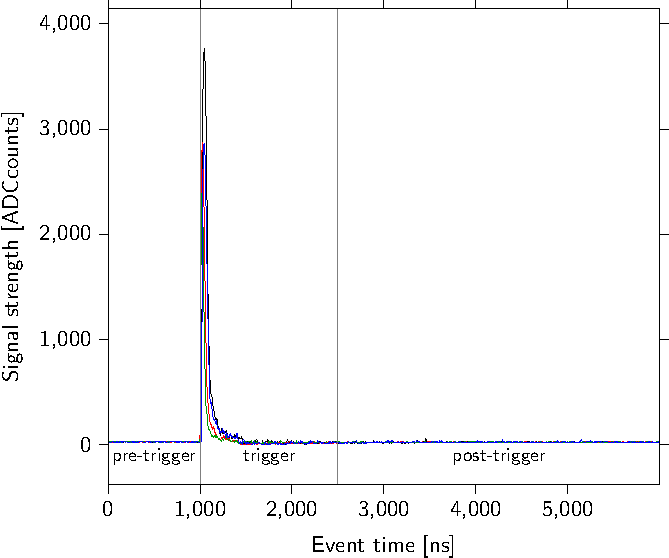
\includegraphics[width=0.6\textwidth]
                    {plots/station/trace_501_1443743701_102112574}
    \caption{Full trace readout of an event, the different trigger windows are indicated.}
    \label{fig:trigger_windows}
\end{figure}

Note that if the \adc alignment is incorrect the same input pulse results in different \adc values for the two \adcs. This makes it more likely for one of the two \adcs to be the first one to cross the thresholds for triggering. By filtering the trace afterwards this bias can be corrected for.


\subsubsection{Trigging for four scintillator detectors}

As mentioned, stations with four scintillator detectors exist, in those cases two \hisparc electronics units are interconnected via UTP cables to provide readout and triggering for four scintillator detectors. When connected the two boxes still work semi-independently, but exchange channel threshold and timing information. Only one of the two (the Master) contains a \gps module, providing it with a very accurate pulse per second (\pps). The \pps is a slower clock than the \SI{200}{\mega\hertz} clock, but it is very accurate. This \pps is used to accurately mark the start of seconds for the fast clock. This \pps is also passed to the Slave unit to synchronise the two clocks. The Master provides the Slave with the current time and a synchronisation pulse. By exchanging threshold information the trigger logic in both the Master and Slave have access to all four channels. Triggers based on four scintillator detectors can then be created. Each unit sends its own data to the PC.


\section{Station}

\subsection{Efficiency of triggering}

% Multiple detector readout with ADCs, use the good timing for coincidence time trigger.
For two scintillator detectors separated by a distance $d$ and sample rate $t_{\mathrm{sample}} = \SI{2.5}{\ns}$ the number of possible (physically relevant) time differences between the two scintillator detectors detecting the same shower front can be calculated by
%
\begin{equation}
    \begin{split}
        t_{\mathrm{max}} &= \frac{d}{c} \\
        n &= \left\lfloor \frac{t_{\mathrm{max}}}{t_{\mathrm{sample}}} \right\rfloor \\
        k &= \{x \in \mathbb{Z} : -n \leq x \leq n \} \\
        \theta_{dt} &= \arcsin \frac{k t_{\mathrm{sample}}}{t_{\mathrm{max}}} \ .
    \end{split}
\end{equation}
%
Here $\theta_{dt}$ is the set of possible angles of the shower axis relative to the line between the detectors. While placing detectors closer together increases the detection efficiency for low energy showers, it decreases the direction reconstruction accuracy.

% An efficient trigger can be made for a certain (and higher) particle density.
Using the equations in \cref{ssec:detection_probability} we can determine the detector distance to efficiently (\SI{>50}{\percent}) detect showers as a function of primary energy. Assume the shower axis is directly between the detectors, since that is where the station will be able to most efficiently detect the shower. The following relation is plotted in \cref{fig:efficiency_distance_energy}, the transition from low efficiency to very efficient is fairly sharp.
%
\begin{equation}
\begin{split}
    r &= \frac{d}{2} \\
    P_2(d) &= \left(1 - \mathrm{e}^{-0.5 \rho(N(E), r)} \right)^2 = 0.5 \ .
\end{split}
\end{equation}
%
So by placing the scintillator detectors \SI{~10}{\meter} apart a \SI{e14.3}{\eV} shower can be detected with \SI{50}{\percent} efficiency if it fell directly between the detectors. At that distance the maximum time difference (assuming a flat shower front) between the detectors is \SI{30}{\ns}. However, shower fronts are not flat, and the rise time of the front can also cause time differences larger than expected from a horizontal shower with a flat front. Since that is a viable possibility the trigger should be long enough to also allow large time differences to detect showers when the detectors are far from the shower core.

\begin{figure}
    \centering
    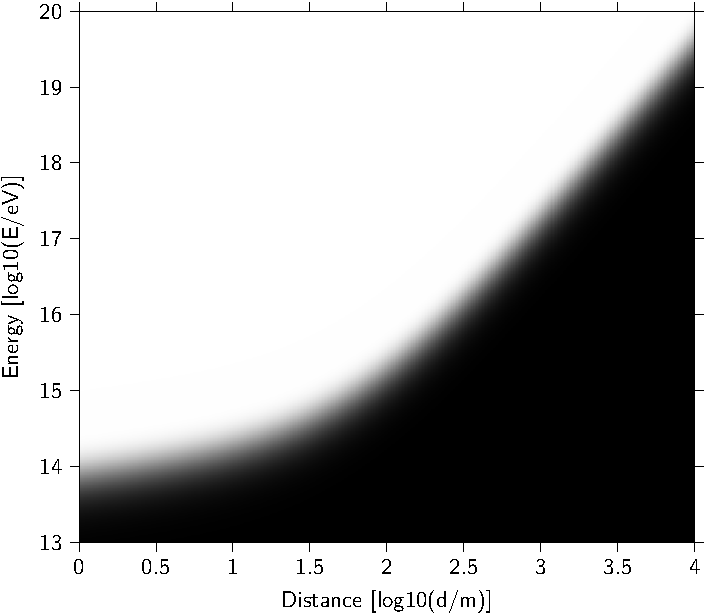
\includegraphics[width=0.6\textwidth]
                    {plots/station/efficiency_distance_energy}
    \caption{Efficiency of detection for showers of various energies as function of distance from the core to the two scintillator detectors. The lines indicate the probability of triggering. The lines indicate \SI{10}{\percent} (dotted), \SI{50}{\percent} (dashed), and \SI{90}{\percent} (solid) probabilities. Below the lines the probability is even lower, while above the top line the probability of detection approaches \SI{100}{\percent}.}
    \label{fig:efficiency_distance_energy}
\end{figure}

% background rate for a given time window
In \cref{fig:temporal_profile} the temporal profile of the shower front was shown, at very large core distances the time difference between the first and last particle may be larger than \SI{3000}{\ns}. For all core distances more than \SI{50}{\percent} of the particles arrive within \SI{1500}{\ns}. This is the value that was chosen as coincidence window for \hisparc. This is long enough to account for most extreme time differences at large core distances. The number of random coincidences due to the muon background (see \cref{eq:background_rate}) with this time window is estimated to be $2 \times \SI{1500}{\ns} \times \left(\SI{0.5}{\meter\squared}\right)^2 \times \left(\SI{200}{\hertz\per\meter\squared}\right)^2 = \SI{0.03}{\hertz}$. In a properly calibrated detector the rate of singles (number of signals over the a threshold per second) are slightly higher, \SI{250}{\hertz} (low) and \SI{120}{\hertz} (high).

The standard trigger setting for a 2-detector station are 2 low signals, the high threshold is ignored. This condition has to be met within the trigger window of \SI{1500}{\ns}. This results in an event rate of approximately \SI{0.33}{\hertz}. Of which a third is expected to be from random coincidences. The low threshold is in the exponential gamma spectrum, a higher \pmt gain will increase the rate of triggers a lot, where at least one of the detectors will have a gamma.

For a 4-detector station the trigger is either 2 high signals or 3 low signals. The same trigger window is used. This results in a trigger rate of approximately \SI{0.66}{\hertz}. Of which about a fifth is expected to be due to random coincidences. The (default) layout of the 4-detector station is described in \cref{sec:station_layout}.

% For (low energy) shower detection a station has multiple detectors close together and contains the trigger logic.
% For high energy showers the density still needs to be high enough in a station for a trigger, this limits maximum core distance for showers.
As noted, the trigger is such that low energy showers are effectively detected by the station and the time window is long enough that it can also trigger on the edges of the shower front from high energy shower.

% Using more than two detectors in a station increases detection efficiency.
% More than two detectors have the possibility of direction reconstruction.
The 4-detector station can more efficiently detect showers, since it has twice the detection area. It will be able to trigger on lower particle densities than a 2-detector station. This makes it capable of detecting large showers from further away. Additionally if three detectors detect a particle it might be possible to reconstruct the direction of the shower axis. This may not be accurate if the station is at the edge of the shower, because the time delays due to the rise time of the shower increase the uncertainty.

% Trigger efficiency as function of core distance and shower energy, for the different triggers (2 in 2-detector, any 2 in 4-detector, and any 3 in 4-detector for reconstructable).
The particle density threshold for triggering on showers with \SI{50}{\percent} efficiency is different for the 2- and 4-detector stations. Also an important value is the trigger efficiency for at least 3-detectors with a hit in the 4-detector station, since this can result in reconstructable showers. In \cref{fig:ldf_energies2} the energy which can be triggered with \SI{50}{\percent} efficiency as a function of core distance is shown for these three cases.

\begin{figure}
    \centering
    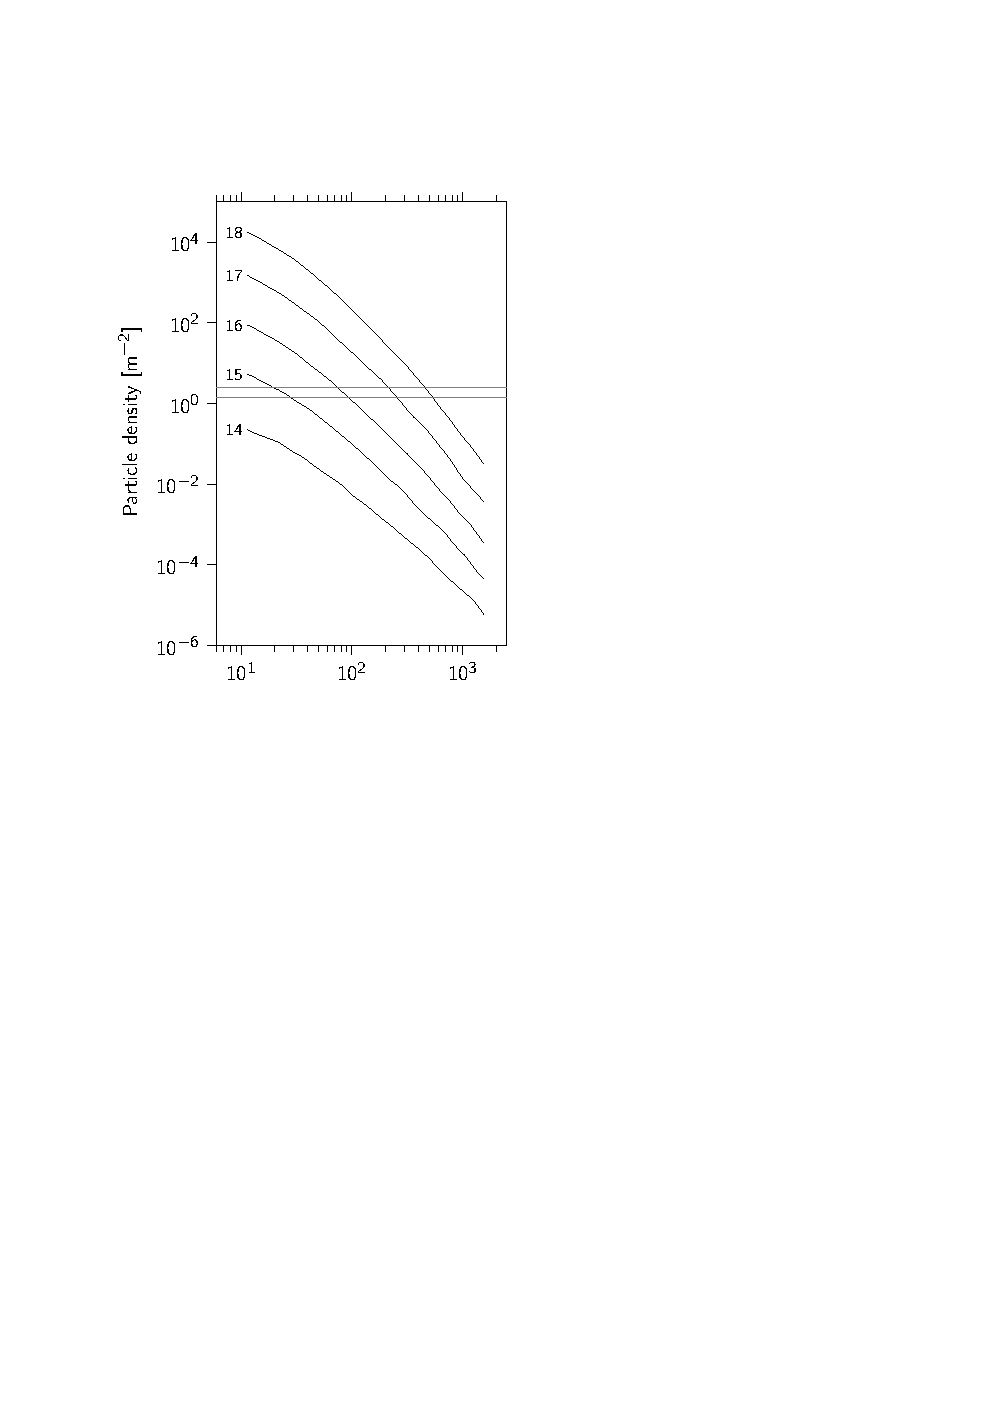
\includegraphics[width=0.5\textwidth]
                    {plots/station/ldf_energies}
    \caption{Trigger efficiency E = \SIrange{e14}{e20}{\eV} showers, add horizontal lines for 2 in 2-detector, any 2 in 4-detector, and any 3 in 4-detector (\SI{50}{\percent} efficient).}
    \label{fig:ldf_energies2}
\end{figure}

\begin{figure}
    \centering
    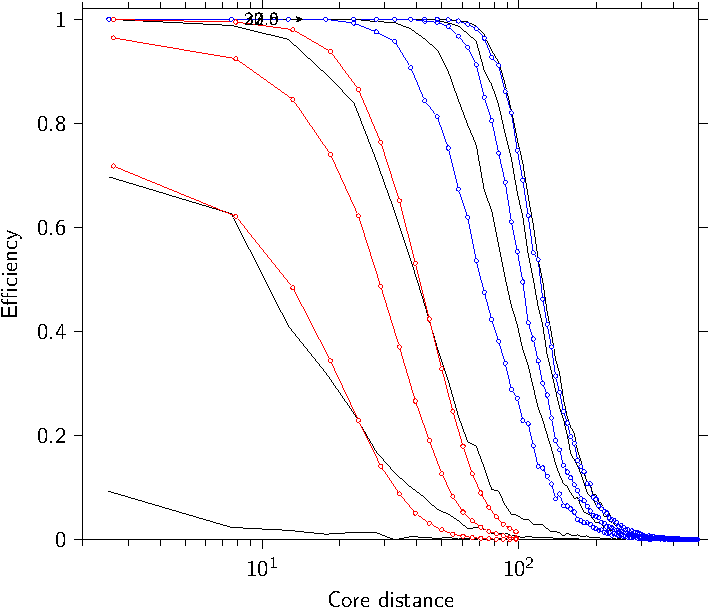
\includegraphics[width=0.6\textwidth]
                    {plots/station/efficiency_two_16}
    \caption{Detection (trigger) efficiency as a function of core distance for showers of different primary energy (and zenith).}
    \label{fig:efficiency_two_16}
\end{figure}


\subsection{Station layout}
\label{sec:station_layout}

% Standard layouts created to encourage uniformity, these are also chosen for good shower acceptance, reconstruction accuracy of station events, and practicality for the locations.
The typical layout of 2-detector stations are relatively straightforward. The two scintillator detectors are separated by \SIrange{6}{10}{\meter}. The \gps antenna is usually placed between the two detectors. The layouts of a typical 4-detector stations are shown in \cref{fig:4_detector_layouts}. The scintillator detectors are separated by \SI{10}{\meter} to exclude the smallest showers and provide accurate direction reconstruction resolution. Given the location of the station is on the roofs of buildings the size of typical roofs also limits the possible size of the stations. The distance between detectors also affects the resolution for reconstructing the direction of air showers. The possible directions for three detectors in an equilateral triangle with \SI{10}{\meter} sides and a timing resolution of \SI{2.5}{\ns} is shown in \cref{fig:discrete_directions}. Using the inner detector with two outer detectors reduces the direction resolution, having only 1/3rd the possible directions. In some cases (space allowing) the decision has been made to move the inner detector outside the triangle to form a second equilateral triangle sharing one of the sides. In this case all combinations of three detectors result in the same possible direction reconstructions.

\begin{figure}
    \centering
    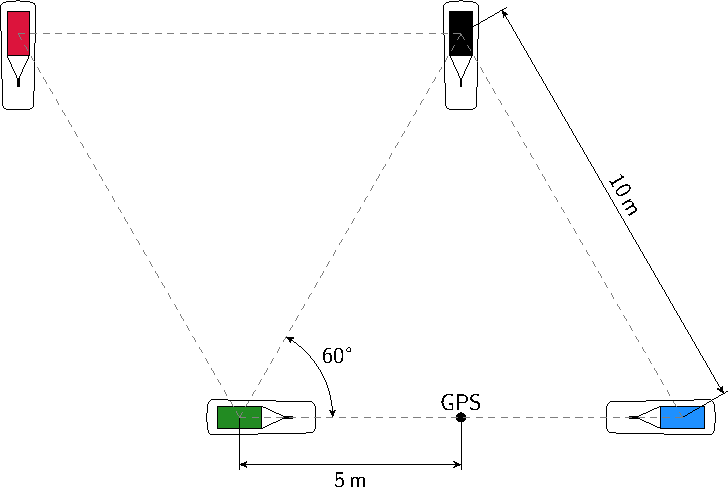
\includegraphics[width=0.4\textwidth]
                    {plots/station/4_detector_diamond}
    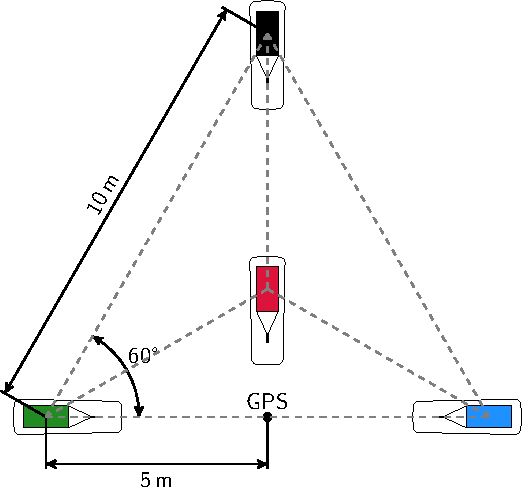
\includegraphics[width=0.4\textwidth]
                    {plots/station/4_detector_star}
    \caption{4-detector station layouts. 4-detector stations are typically placed in the diamond or star formation. Both contain multiple triangles between sets of 3 detectors.}
    \label{fig:4_detector_layouts}
\end{figure}

\begin{figure}
    \centering
    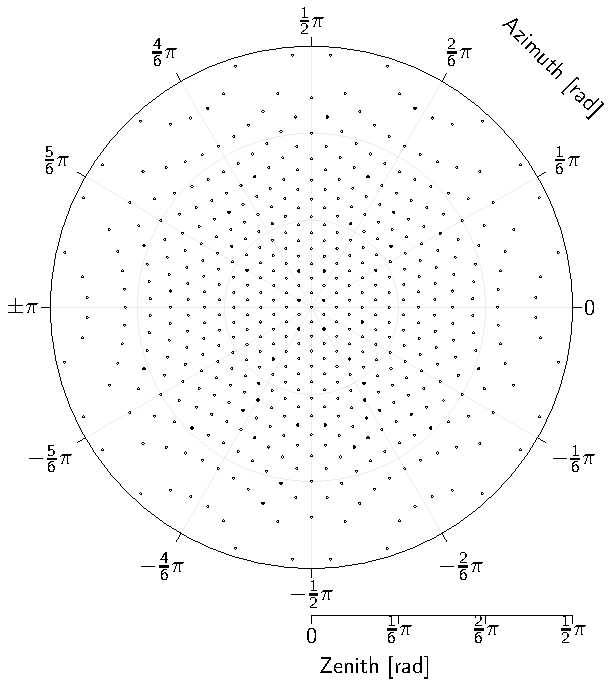
\includegraphics[width=0.6\textwidth]
                    {plots/station/discrete_directions}
    \caption{Both 4-detector layouts result in the following distribution of possible shower directions given \SI{2.5}{\ns} arrival time sampling in the detectors. For the diamond layout more points can be made by more combinations, i.e. more possible solutions. Approximately \SI{5}{\degree} between adjacent points near Zenith.}
    \label{fig:discrete_directions}
\end{figure}

The layout of each station is not always precisely according to the suggested layout. Not all roofs provide the required space. It is not a problem if the layout deviates from the suggested ones, as long as the actual positions are known. In order to get the absolute position of the detectors their positions are measured relative to the \gps antenna, whose position is known. \gps positions are automatically submitted by the station to the datastore. From the \gps the distance to and the angle between (True?) North and the center of each scintillator is measured. Additionally, the rotation of the long side of the scintillator to North can be recorded, though this is less important. The used coordinate system is described in more detail in \cref{ch:coordinates}. If the location of detectors relative to the \gps is changed the new layout can be recorded with the timestamp of when it changed. The data analysis takes these changes into account to use the correct layout when reconstructing events. For students a document has been created which outlines the steps for measuring the layout of their station and how they can submit them to \hisparc. Information about the position of scintillator detectors in 2-detector stations is also important. Even though full direction reconstruction is not possible with only two detection points it can be used to define a plane where the shower should come from \cite{schultheiss2016pair}.

In \cref{fig:locations_501} the different \gps and scintillator detector locations for station 501 are shown. The outlier \gps locations are caused by the usage of temporary \gps antenna during tests. The station layout described by the clustered positions describes the original star-layout, an equilateral triangle with one scintillator detector in the center. When station 510 was built station 501 was also moved to create overlapping diamond-shaped stations. One detector (green) was not moved during this transition. For each physical \gps location (including the temporary test locations) the relative scintillator detector positions have been measured. Other Science Park stations for which the detectors have been moved are 502 and 505. For station 505 this was done multiple times because alterations to the roof on which the scintillator detector reside required them to be moved.

\begin{figure}
    \centering
    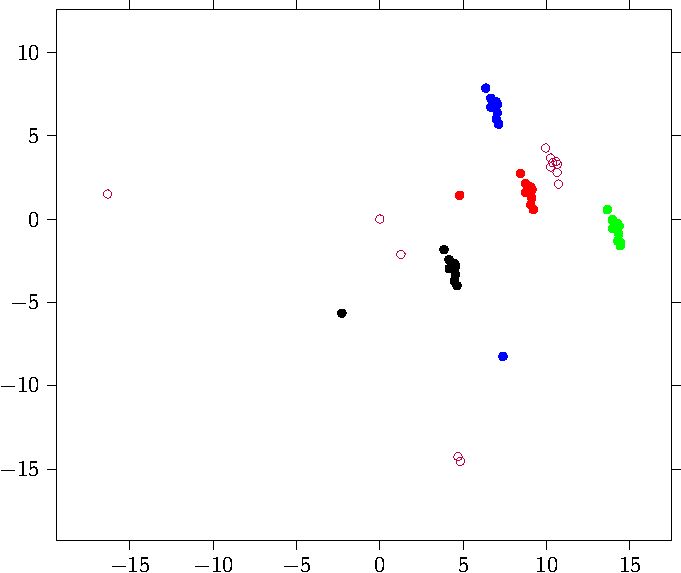
\includegraphics{plots/station/locations_501}
    \caption{Detector (closed circles) and \gps locations (open circles) for station 501. Over time the detectors and \gps antenna for station 501 have been moved multiple times. The clusters of circles are not necessarily movements of the \gps or the scintillator detectors but merely new self-surveys by the \gps resulting in a slightly different position.}
    \label{fig:locations_501}
\end{figure}


\subsection{Scintillator detector timing offsets}

Assuming cosmic rays arrive from all direction isotropically then the distribution of detection time difference between two scintillator detectors should be symmetric around \SI{0}{\ns}. Because for each zenith angle an equal amount of showers come from all azimuthal angles. The distribution of measured time differences for one day of data is shown in \cref{fig:detector_time_difference_distribution}. The average value of the observed distribution is often slightly offset from \SI{0}{\ns}. This may be caused by different transit times in the \pmt and signal travel time in the cables.

\begin{figure}
    \centering
    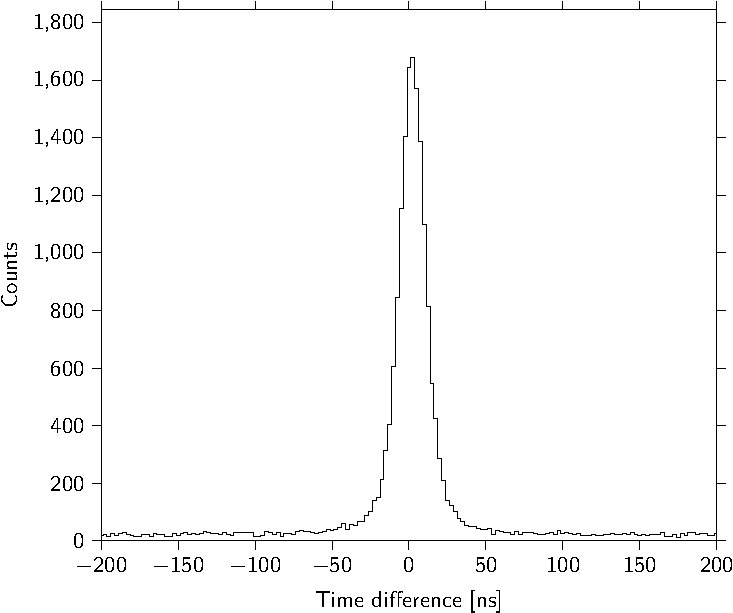
\includegraphics{plots/station/detector_time_difference_distribution}
    \caption{This shows the distribution of arrival time differences between the two scintillator for triggered events. A days worth of data is used. The peak around \SI{0}{\ns} are from strongly correlated particles, most events with time differences larger than \SI{100}{\ns} are for random coincidences.}
    \label{fig:detector_time_difference_distribution}
\end{figure}

The offsets between detectors in a station can be very stable over time. Changes to the station hardware and configuration can disrupt this. In \cref{fig:detector_offset_drift_month_501} the detector offsets for a 4-detector station are shown. The large jumps in offsets are explained by the change to \hisparciii electronics.

\begin{figure}
    \centering
    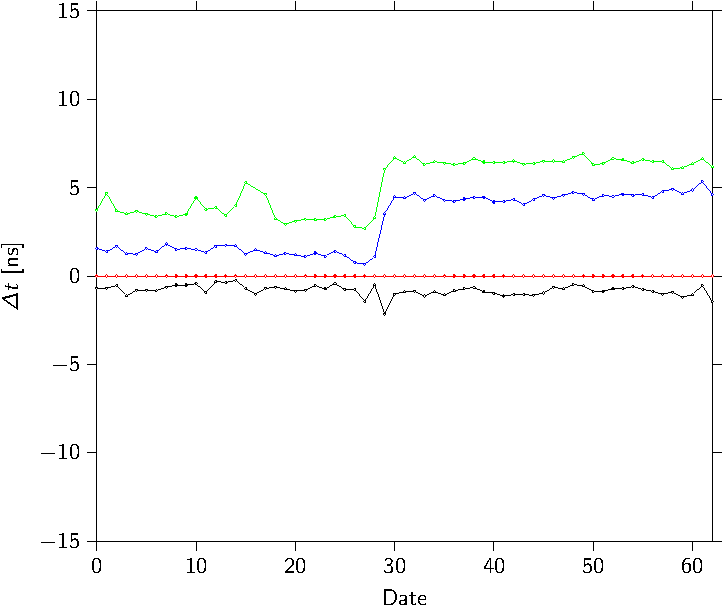
\includegraphics{plots/station/detector_offset_drift_month_501}
    \caption{This shows the changes in scintillator detector offsets for the scintillator detectors of station 501. Scintillator detector 2 (red) is used as reference. Scintillator detector 1 (black) is the other channel connected to the Master electronics. The large jump observed for detector 3 (green) and 4 (blue) was caused by the switch from \hisparcii to \hisparciii electronics.}
    \label{fig:detector_offset_drift_month_501}
\end{figure}

These detector offsets are automatically determined each day for each station. In \cref{fig:detector_offset_distribution} the distribution of the offset between the two detectors connected to the Master electronics is shown. The mean offset is \SI{0.02 \pm 0.30}{\ns} and the width of the distribution is \SI{2.31 \pm 0.24}{\ns}. The distribution between Master and Slave is more offset with a mean of \SI{1.00 \pm 0.60}{\ns} with approximately the same width \SI{2.25 \pm 0.84}{\ns}.

\begin{figure}
    \centering
    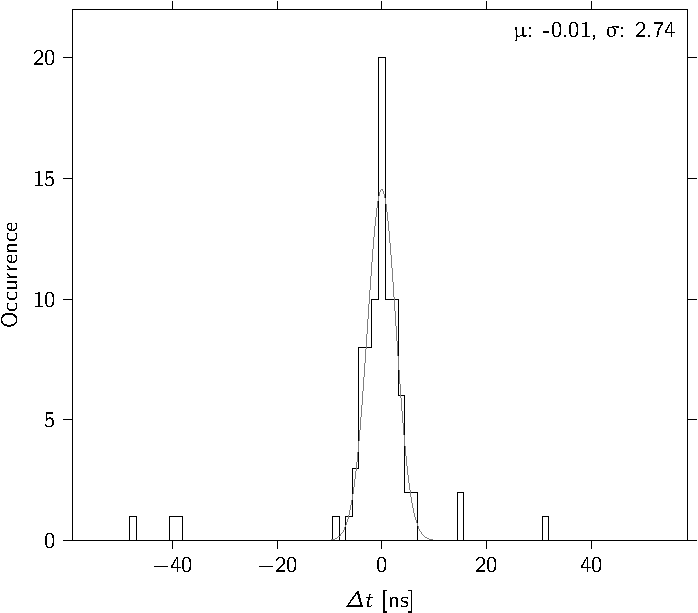
\includegraphics{plots/station/detector_offset_distribution}
    \caption{Distribution of scintillator detector offsets. The scintillator detector offsets between the two scintillator detectors connected to the Master electronics for all \hisparc stations are shown.}
    \label{fig:detector_offset_distribution}
\end{figure}


\subsubsection{Master slave timing}
\label{sec:masterslavetiming}

The offset between Master and Slave scintillator detectors may be caused by delays in the exchange of threshold information. The Master and Slave separately determine if a trigger occurred, determine the event timestamp, and  transmit it to the \daq software. In the \daq software the events from the Master and Slave are combined again (using the timestamp to find those that belong together) and the timestamp from the Master is used for the event. However, a slight timestamp difference may exist. In \cref{fig:time_delta_501} the distribution of timestamp differences for \num{6624} events is shown. This timestamp difference could be used to partly compensate for time offsets between the Master and Slave scintillator detectors. However, simply fitting the overall time difference compensates for this offset and individual scintillator detector offsets. The timestamp difference could be used on an event to event basis to improve the time resolution. But this is found to hardly improve the arrival time accuracy (\SI{0.5}{\ns}). Moreover, timestamp difference data is unavailable available for practically all \hisparc data. This effect slightly increases the arrival time difference accuracy between Master and Slave scintillator detectors, the mean offset is compensated for.

\begin{figure}
    \centering
    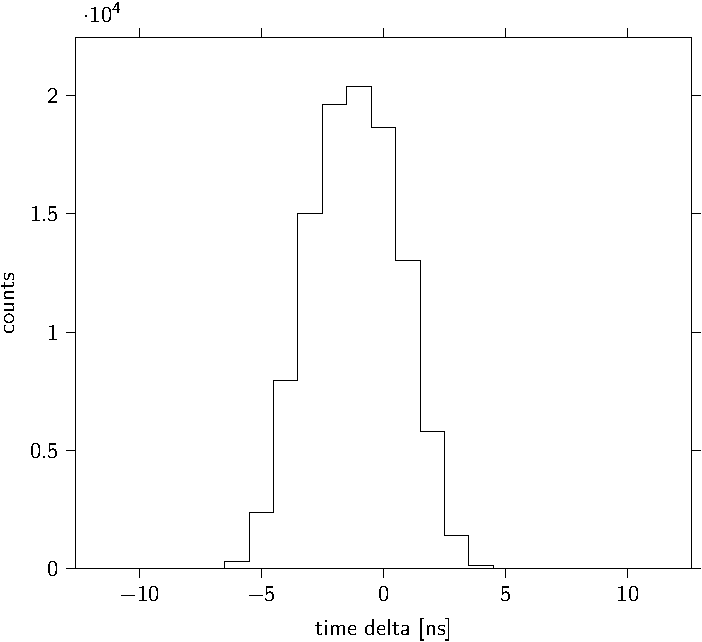
\includegraphics{plots/station/time_delta_501}
    \caption{Timestamp difference distribution between the Master and Slave, trigging on the same events but making their own timestamps. The mean offset is \SI{-2.0}{\ns} and the width of the distribution is \SI{2.0}{\ns}.}
    \label{fig:time_delta_501}
\end{figure}


\subsection{Shower direction reconstruction}

% Explain simple direction reconstruction with 3 detection points (flat/curved shower).
When there are three detection points (which are not on a line) the shower axis direction can be constrained. In this case the detectors are assumed to be at the same height and the shower front is considered to be thin and flat, an approximation which can be valid close to the core and at the short distances between detectors as they occur in a station. The 2-dimensional flat-front reconstruction method for three detection points is described in \cite{fokkema2012hisparc}. The following equations result in the shower axis direction, i.e. the azimuth ($\phi$) and zenith ($\theta$).

\begin{equation}
    \label{eq:direction-2dflat}
    \begin{split}
        \phi &= \arctan \left(\frac{r_1 \Delta t_2 \cos \phi_1 - r_2 \Delta t_1 \cos \phi_2}{r_2 \Delta t_1 \sin \phi_2 - r_1 \Delta t_2 \sin \phi_1} \right) \ , \\
        \theta &= \arcsin \left(\frac{c \Delta t_i}{r_i \cos(\phi - \phi_i)} \right) \ .
    \end{split}
\end{equation}

Here $r_i$ is the distance between detector 0 and detector $i$, $\Delta t_i$ is the time difference between detector 0 and detector $i$, and $\phi_1$ the angle between East and detector $i$ as seen from detector 0. Note that care must be taken to take the correct quadrant for the $\arctan$ and that $\phi - \phi_i \ne 2 \pi$. The same results can be achieved with a Cartesian approach as described in \cite{montanus2015direction}. This gives

\begin{equation}
    \label{eq:direction-2dflat}
    \begin{split}
        \phi &= \arctan \left(\frac{-u_x v_z}{u_y v_z} \right) \ , \\
        \theta &= \arcsin \left(\sqrt{\frac{u_x^2+u_y^2}{v_z^2}} \right) \ .
    \end{split}
\end{equation}

Here $u_x = \Delta t_2 x_1 - \Delta t_1 x_2$, $u_y = \Delta t_2 y_1 - \Delta t_1 y_2$, and $v_z = x_1 y_2 - x_2 y_1$. The $x$ and $y$ coordinates are as defined by the ENU coordinate system described in \cref{ch:coordinates}, in this case using detector 0 as reference.


\subsection{Performance of a station}

The reconstruction accuracy of a single \hisparc station was tested at the \kascade experiment. A 4-detector \hisparc station was placed between the \kascade detectors and triggered (using an external trigger) when the surrounding \kascade detectors detected an event. The \kascade reconstruction of the shower which triggered the \hisparc station were made available. By reconstructing the \hisparc data and comparing this to the \kascade reconstruction the performance of a single station is tested.


\subsubsection{Direction reconstruction accuracy}

The reconstruction of the shower direction has shown to be accurately reconstructable. The results reported in \cite{fokkema2012hisparc} are shown in \cref{fig:angle_kascade_core_distance}. Depending on the core distance of the shower and the overall particle density. The uncertainty is lower for showers with the core close to the station, quickly increasing with distance. If only large showers were selected, higher particle density, than the uncertainty remains lower at larger core distances.

\begin{figure}
    \centering
    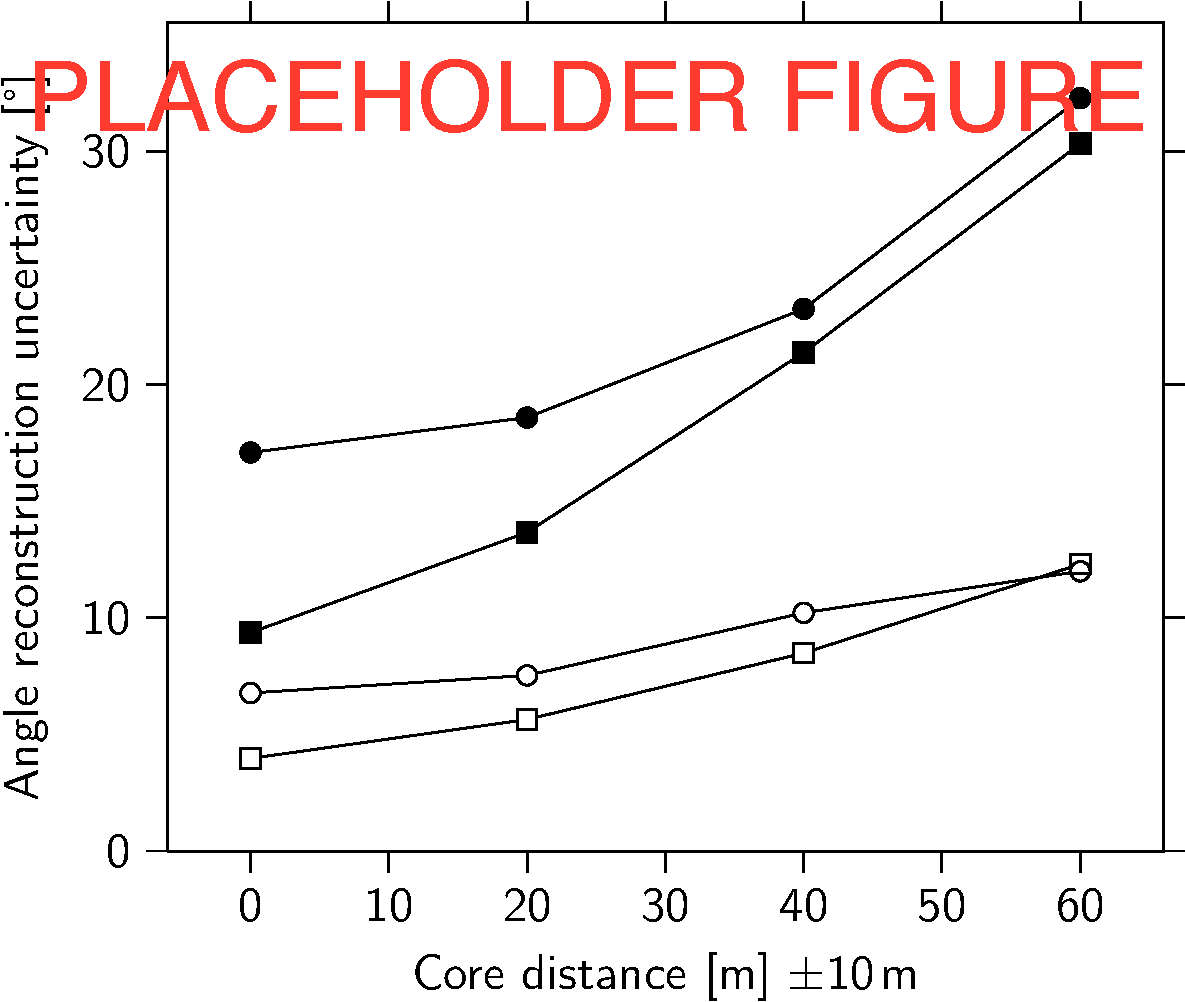
\includegraphics[width=0.6\textwidth]
                    {plots/station/angle_kascade_core_distance}
    \caption{Test station at KASCADE was used to verify the performance of a single station. The direction agreement between simultaneously detected events is shown. The azimuth (closed) and zenith (open) reconstruction uncertainties from the data (squares) are compared to simulations (circles). At increased core distances the effects of the shower rise time cause the uncertainty to rise quickly.}
    \label{fig:angle_kascade_core_distance}
\end{figure}


\subsubsection{Density reconstruction accuracy}
\label{sec:kascade_density}

The \hisparc scintillator detectors detect particles, and via the pulse integral an estimation can be made for the number of detected particles. The desired value is the actual particle density on of the shower front at the location of the detector. However, there is no perfect answer, different particle densities can result in the same number of detected particles. Using Bayes' Theorem the probability that the actual particle density is $\lambda$ given a measurement $x$ is given by
%
\begin{equation}
    \label{eq:bayes_poisson}
    P(\lambda|x) = P(x|\lambda) P(\lambda) / \alpha_0
\end{equation}
%
where $P(x|\lambda)$ is the Poisson distribution given in \ref{eq:poisson}. $P(\lambda)$ is the Bayesian prior function, which is the \emph{a priori} assumed distribution of possible values for $\lambda$, and $\alpha_0$ is a normalisation constant given by $\int_0^\infty P(x|\lambda) P(\lambda) \ud \lambda$. \cite{vulpen2011poisson}. For $P(\lambda)$ the distribution of values is taken as the distribution of \kascade predictions. Due to the required triggering of the \kascade detector for data to be recorded and the applied data cuts the probability of a very low particle density is suppressed.

Using \cref{eq:bayes_poisson} a relation between the detected number of particles and the contributions from the actual particle densities is obtained. This is shown in \cref{fig:poisson_ranges}. From this we can see that if \num{10} particles are detected there is a \SI{50}{\percent} chance that this is caused by an actual density of \num{8.3} particles or less.

\begin{figure}
    \centering
    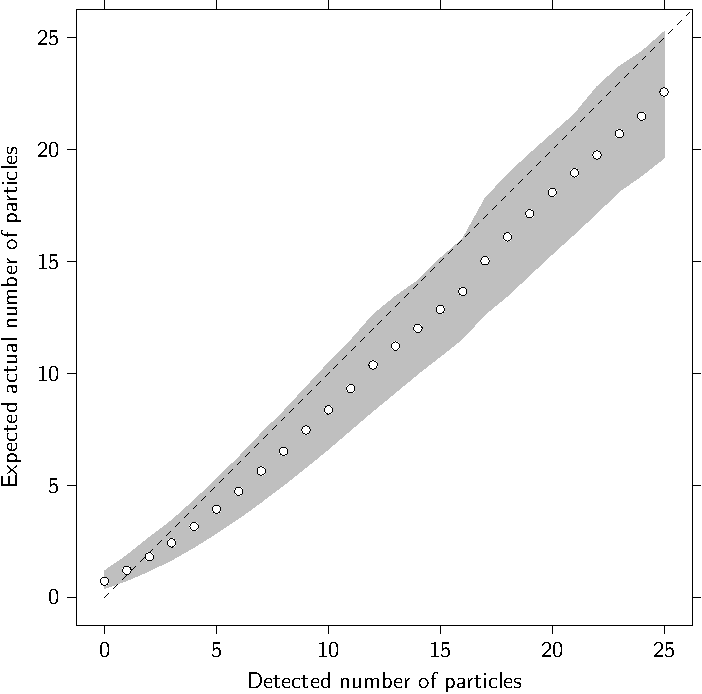
\includegraphics[width=0.6\textwidth]
                    {plots/station/poisson_ranges}
    \caption{For a given number of detected particles the probability distribution that this number was caused by a certain actual particle density is shown. The median value of the distribution (solid, black) is indicated. The shaded area contains \SI{50}{\percent} of the distributions, evenly distributed around the median. For reference the $y = x$ line (dashed) is shown.}
    \label{fig:poisson_ranges}
\end{figure}

In \cref{fig:hisparc_kascade_station_mpv} the by \kascade determined particle density at the station is compared to the measured signal. The \kascade experiment has many detectors to accurately measure the shower front, it then fits an \ldf to this, taking the shower inclination into account, and calculates the expected particle densities in the shower front at each of the \hisparc scintillator detectors. For this analysis the particle densities are converted to particle densities on the ground using $\rho^\prime = \cos\theta(\rho_{\Pe} + \rho_{\Pmu})$, compensating for the effective area. No error is given for the \kascade determined particle density, so it is assumed to be correct. However, the \ldf inherently predicts a smooth radially symmetric density distribution, but actual showers have local minima and maxima. The uncertainty is large at low particle densities due to the scintillator detector signal transmission efficiency and Poisson effects. At high particle densities the non-linearity of the \pmt is the main source of uncertainty.

The scintillator detector error is estimated by a Gaussian distribution with a width of $\sigma = \sqrt{\rho} 0.68$, the error increases at higher densities.
%The error due to the non-linearity is estimated by $\sigma_{V_{\mathrm{out}}} = \sigma_{V_{\mathrm{in}}} \frac{\mathrm{d}V_{\mathrm{out}}}{\mathrm{d}V_{\mathrm{in}}}$.

\begin{figure}
    \centering
    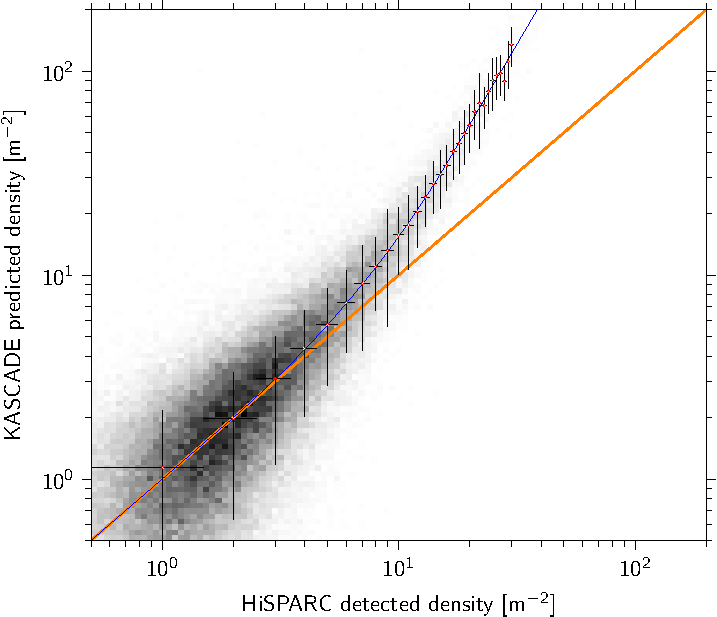
\includegraphics[width=0.6\textwidth]
                    {plots/station/hisparc_kascade_station_mpv}
    \caption{Test station at KASCADE was used to verify the particle density measurement of the scintillator detectors. Here the reconstructed station average particle density is compared to the KASCADE predicted particle density. The non-linearity of the \pmts cause an underestimation of the \hisparc particle density (blue, solid), compressing the value range at higher signal strength, the Poisson errors are also compressed, as can be seen in the predicted error (green, dashed). The errors due to scintillator detector effects (red, dashed) and \pmt saturation (blue, dashed) are also indicated [todo clearly show all errors, perhaps 2d Hist in separate plot].}
    \label{fig:hisparc_kascade_station_mpv}
\end{figure}

% Shower core/energy determination impractical with single station.
Determination of the shower core is impractical with a single station. The error on the determination of the particle density is to high and the number of detection points to low.


\section{Weather station}

% Optional weather station to provide local weather data.
Optionally a \hisparc station can be extended with a weather station to provide local weather measurements. These measurements can help in understanding how shower development is affected by atmospheric conditions. For instance an high air pressure increases the number of collisions in air showers, thereby reducing the number of particles that reach sea level. This lowers the trigger rate for a station. Additionally some of the scintillator detector components have efficiencies dependent on their temperature. By measuring the temperature detections may be corrected for the changed efficiency. \hisparc uses a Davis Vantage Pro 2 weather station \cite{davis2012vantagepro} which includes the following sensors; temperature, relative humidity, atmospheric pressure, wind direction, wind speed, solar radiation, UV index and rain rate. These sensors are readout at a \SI{5}{\second} interval. The weather station is described in more detail in \cite{devries2012weather}. Currently there are 19 \hisparc stations that also have a weather station.

\begin{figure}
    \centering
    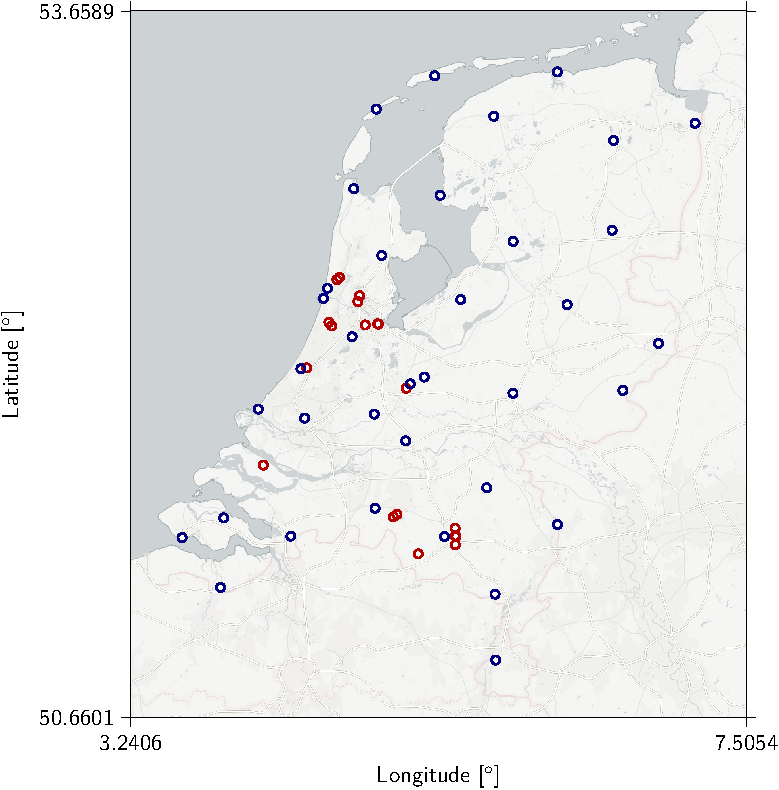
\includegraphics[width=0.6\textwidth]
                    {plots/station/map_weather_knmi}
    \caption{Locations of \hisparc weather stations (red) and the KNMI weather stations (blue).}
    \label{fig:map_weather_knmi}
\end{figure}

% May not be required at each station, can use freely available KNMI data. However, in some cases closest KNMI station is far away.
Note that it is not required for all stations to have a weather station. The Royal Dutch Meteorological Institute (\knmi) also provides a public weather data service in the Netherlands. \knmi has 36 stations spread in a regular grid around the Netherlands. Not all \hisparc stations are close to a \knmi station, for some weather quantities this is no problem because they are similar over long distances, or can be interpolated. Besides temperature the local solar radiation strongly influences the temperature of the detector in a ski-box. The location of \hisparc and \knmi weather stations are shown on the map in \cref{fig:map_weather_knmi}.


\section{Durability}
\label{sec:detector-durability}

One of the issues that may arrise during or after the construction of the scintillator detector are light leaks. As the name suggests this means that light from outside can leak into the detector causing false readings. These are often directly evident after construction, although some develop over time when the detector was improperly wrapped. A light leak causes may small pulses in the channel of the leaking scintillator detector. This causes an increase in the event rate, however, 4-detector stations are less affected because of the trigger settings. The number of small peaks in the 4-detector station event do increase. This problem is often easily fixed by applying extra pond foil and tape.

The connection between the scintillator and lightguide (glue) is known to have broken on occasion, the scintillator detector may still works but with lower efficiency. As long as the detector is not moved and properly supported it can continue to operate indefinitely. Repairing the scintillator detector takes almost as much time as the initial construction, and has to be done very carefully to prevent damaging the attached \pmt.

In the small time period shown in \cref{fig:temperature_timeline} temperatures above \SI{42}{\degreeCelsius} are seen. The specifications of the \pmt state its maximum operational temperature as \SI{60}{\degreeCelsius}. Such high temperatures may occur occasionally. However, this does not seem to be an issue yet.

A batch of \pmts has been encountered where the failure rate was very high, around 30 \pmts failed. This is quite a significant number since \hisparc has approximately 300 \pmts in use. The power supplies of these \pmts failed. The actual vacuum tubes were still working fine. The costs to have the power supply replaced by the manufacturer were excessive, almost equal to a new \pmt. This was one of the motivations to manufacture the \nikhef \pmt power supplies. Replacing \pmts is a fairly easy process and can be performed without moving the scintillator detector.

The power supplies provided with the \hisparc electronics by the manufacturer were from a bad batch. All have failed within a couple months of use. These have been replaced by a different type of power supply of which no failures have yet been observed. Not all electronics were deployed at once, so preemptive power supply replacements have been done for those deployed later.

On some occasions power interruptions can cause down time for a station.  There are cases where supplies were disconnected by cleaning crews or students that wanted to use the power socket for their own devices. Some schools disable their power grid during vacation time, in order to save power. Usually the station resumes operation after the vacation when the power is restored.

Despite these possible problems most detectors perform perfectly for many years, and problems can be addressed easily, as was the goal. One example of a perfectly performing station is station 13 at Hervormd Lyceum West in Amsterdam. This station has been working since March 2005 with minimal interruptions, it has currently detected \num{e8} events.
